\chapter{Results}
\label{chap:results}

\begin{quotation}
	\noindent ``Without data, you are just another person with an opinion.''
\end{quotation}
\begin{flushright}
	- W. Edwards Deming
\end{flushright}

\noindent
All the required background information on all the elements relevant to the empirical process have been presented in Chapters~\ref{chap:anns}-\ref{chap:probability}. The proposed \acf{BHH} was presented in Chapter~\ref{chap:bhh} and the design and methodology of the empirical process was presented in Chapter~\ref{chap:methodology}. The methodology presented a number of experiments to conduct, including a case study on the behaviour of the \acs{BHH} during training, and a comparison to the performance of state-of-the-art, standalone, low-level \index{heuristic}heuristics. The methodology also defined a number of experiments related to the empirical testing of the effects of hyper-parameters on the outcomes of the \acs{BHH}.

Finally, this chapter provides the outcome of these empirical processes and provides results on all the experiments that have been conducted. Detailed discussions follow on the outcomes of each experiment. Discussions are accompanied by figures and plots to help provide visual aid for the discussions. The output of the statistical analysis that yielded the results presented in the chapter is provided in Appendix~\ref{app:statistical_analysis}. The remainder of the chapter is structured as follows.

\begin{itemize}
	\item \textbf{Section \ref{sec:results:case_study}} provides detailed discussions on the outcomes of the case study on the behaviour of the \acs{BHH}. Illustrations are provided to show the outcomes of the learning process of the \acs{BHH}, while training the underlying \acf{FFNN}.

	\item \textbf{Section \ref{sec:results:bhh_vs_low_level_heuristics}} provides the results of the performance of the \acs{BHH} compared to individual low-level \index{heuristic}heuristics as it relates to all datasets. Three variants of the \acs{BHH} are included in these results. These include the baseline configuration, as well as a configuration that only includes gradient-based \index{heuristic}heuristics in the \index{heuristic pool}heuristic pool, and a configuration that only includes meta-heuristics in the \index{heuristic pool}heuristic pool.

	\item \textbf{Section \ref{sec:results:bhh_variant_hp}} provides the results for the experimental group that analyses the effects of the \index{heuristic pool}\textit{heuristic pool} hyper-parameter on the outcomes of the \acs{BHH}.

	\item \textbf{Section \ref{sec:results:bhh_variant_population}} provides the results for the experimental group that analyses the effects of the \textit{population size} hyper-parameter on the outcomes of the \acs{BHH}.

	\item \textbf{Section \ref{sec:results:bhh_variant_credit}} provides the results for the experimental group that analyses the effects of the \textit{credit assignment strategy} hyper-parameter on the outcomes of the \acs{BHH}.

	\item \textbf{Section \ref{sec:results:bhh_variant_reselection}} provides the results for the experimental group that analyses the effects of the \textit{reselection interval} hyper-parameter on the outcomes of the \acs{BHH}.

	\item \textbf{Section \ref{sec:results:bhh_variant_replay}} provides the results for the experimental group that analyses the effects of the \textit{replay window size} hyper-parameter on the outcomes of the \acs{BHH}.

	\item \textbf{Section \ref{sec:results:bhh_variant_reanalysis}} provides the results for the experimental group that analyses the effects of the \textit{reanalysis interval} hyper-parameter on the outcomes of the \acs{BHH}.

	\item \textbf{Section \ref{sec:results:bhh_variant_burn_in}} provides the results for the experimental group that analyses the effects of the \textit{burn in window size} hyper-parameter on the outcomes of the \acs{BHH}.

	\item \textbf{Section \ref{sec:results:bhh_variant_normalise}} provides the results for the experimental group that analyses the effects of the \textit{normalisation} hyper-parameter on the outcomes of the \acs{BHH}.

	\item \textbf{Section \ref{sec:results:bhh_variant_discounted_rewards}} provides the results for the experimental group that analyses the effects of the \textit{discounted rewards} hyper-parameter on the outcomes of the \acs{BHH}.

	\item \textbf{Section \ref{sec:results:overfitting}} provides a brief discussion on overfitting as it is observed for some of the empirical tests.

	\item \textbf{Section \ref{sec:results:practical_applications}} provides a brief discussion on the practical application of the \acs{BHH} to real-world problems.

	\item \textbf{Section \ref{sec:results:summary}} provides a brief summary of the chapter.
\end{itemize}

\section{Behavioural Case Study}\label{sec:results:case_study}

%%%%%%%%%%%%%%%%%%%%%%%%%%%%%%%%%%%%%%%%%%%%%%%%%%%%%
% METRICS
%%%%%%%%%%%%%%%%%%%%%%%%%%%%%%%%%%%%%%%%%%%%%%%%%%%%%


\begin{figure}[htpb]
	\centering
	\includegraphics[width=1.0\textwidth]{case_study/metrics/figures/train/train_loss.pdf}
	\caption{The average training loss over 30 epochs, obtained from 30 runs of the case study on the behaviour of the \acs{BHH} on the Iris dataset, illustrated in log scale.}
	\label{fig:results:case_study:train_loss}
\end{figure}

\begin{figure}[htpb]
	\centering
	\includegraphics[width=1.0\textwidth]{case_study/metrics/figures/test/test_loss.pdf}
	\caption{The average test loss over 30 epochs, obtained from 30 runs of the case study on the behaviour of the \acs{BHH} on the Iris dataset, illustrated in log scale.}
	\label{fig:results:case_study:test_loss}
\end{figure}

\begin{figure}[htpb]
	\centering
	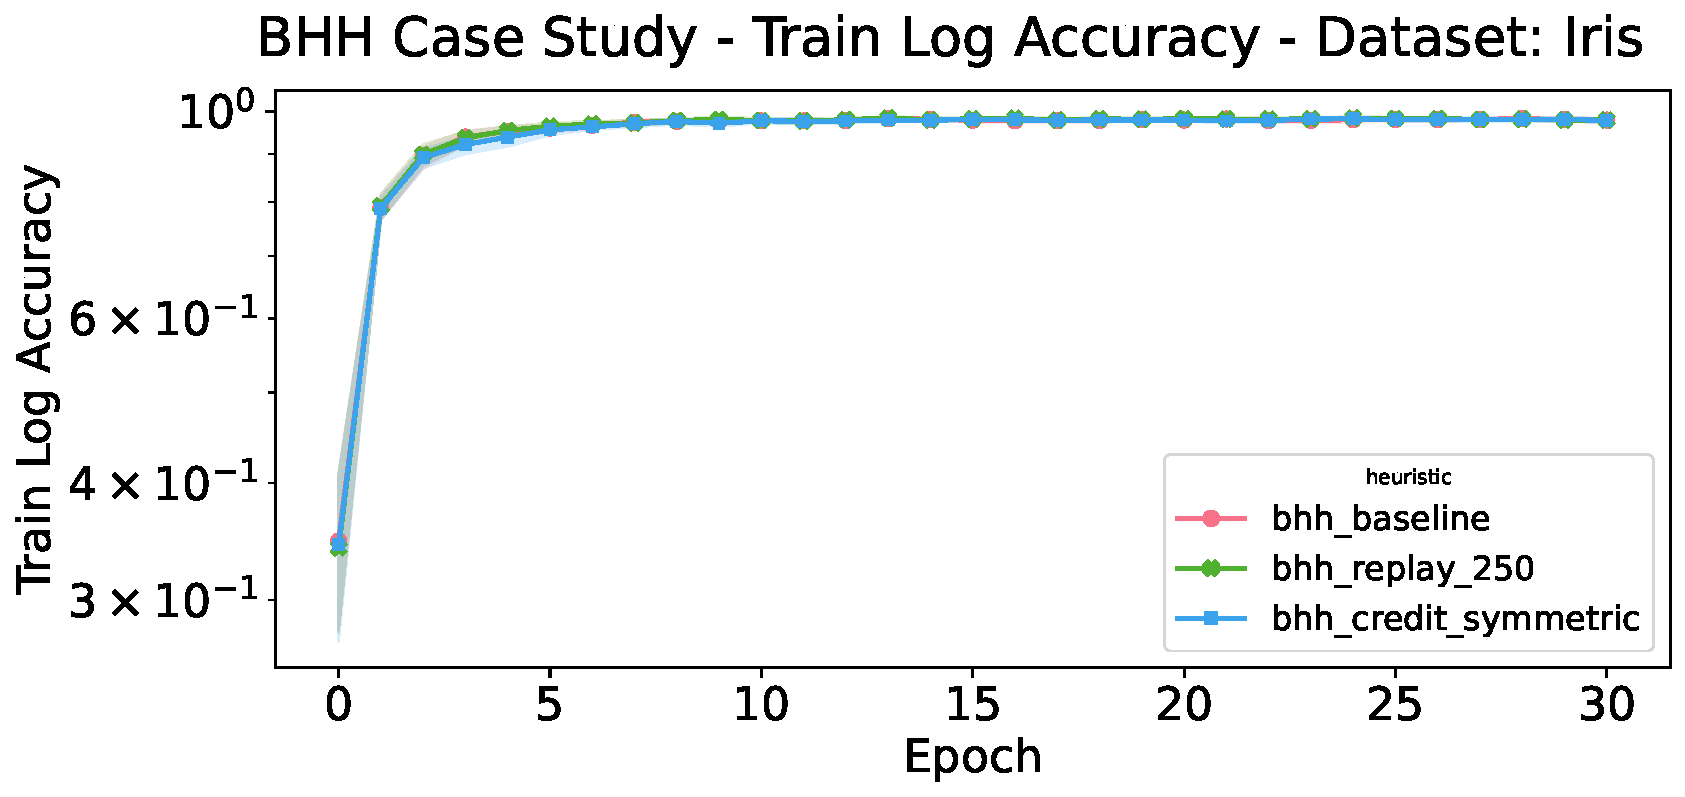
\includegraphics[width=1.0\textwidth]{case_study/metrics/figures/train/train_accuracy.pdf}
	\caption{The average training accuracy over 30 epochs, obtained from 30 runs of the case study on the behaviour of the \acs{BHH} on the Iris dataset, illustrated in log scale.}
	\label{fig:results:case_study:train_accuracy}
\end{figure}

\begin{figure}[htpb]
	\centering
	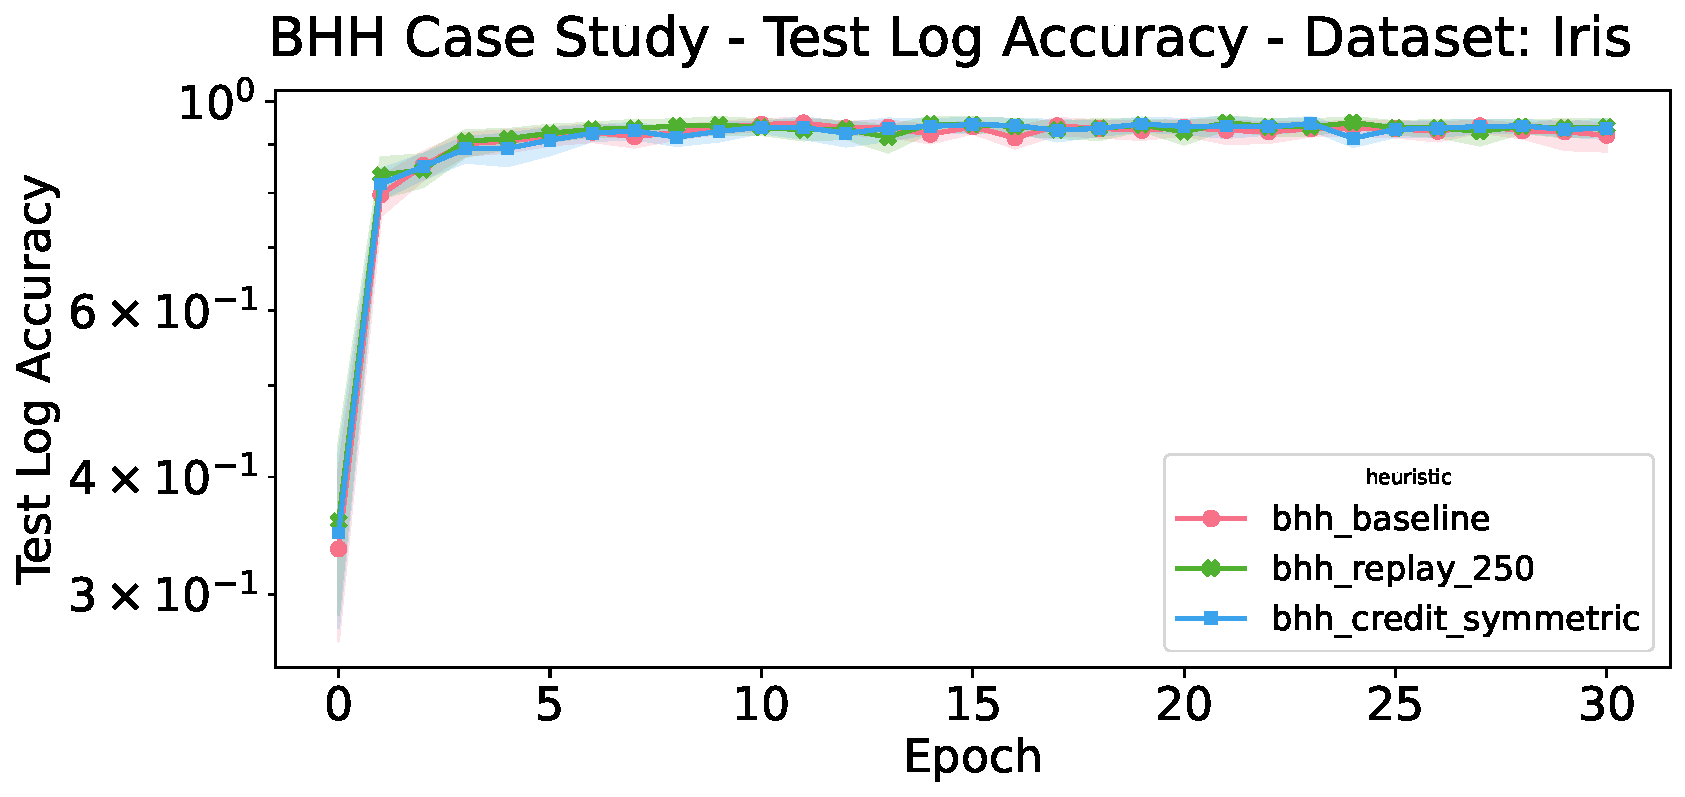
\includegraphics[width=1.0\textwidth]{case_study/metrics/figures/test/test_accuracy.pdf}
	\caption{The average test accuracy over 30 epochs, obtained from 30 runs of the case study on the behaviour of the \acs{BHH} on the Iris dataset, illustrated in log scale.}
	\label{fig:results:case_study:test_accuracy}
\end{figure}


%%%%%%%%%%%%%%%%%%%%%%%%%%%%%%%%%%%%%%%%%%%%%%%%%%%%%
% PARAMS ALPHAS
%%%%%%%%%%%%%%%%%%%%%%%%%%%%%%%%%%%%%%%%%%%%%%%%%%%%%


\begin{figure}[htpb]
	\centering
	\includegraphics[width=1.0\textwidth]{case_study/params/figures/alphas/alpha[0].pdf}
	\caption{The average value of the concentration parameter $\alpha_{0}$ (\acs{SGD}) over 250 training steps, obtained from 30 runs of the case study on the behaviour of the \acs{BHH} on the Iris dataset, illustrated in log scale.}
	\label{fig:results:case_study:alpha:0}
\end{figure}

\begin{figure}[htpb]
	\centering
	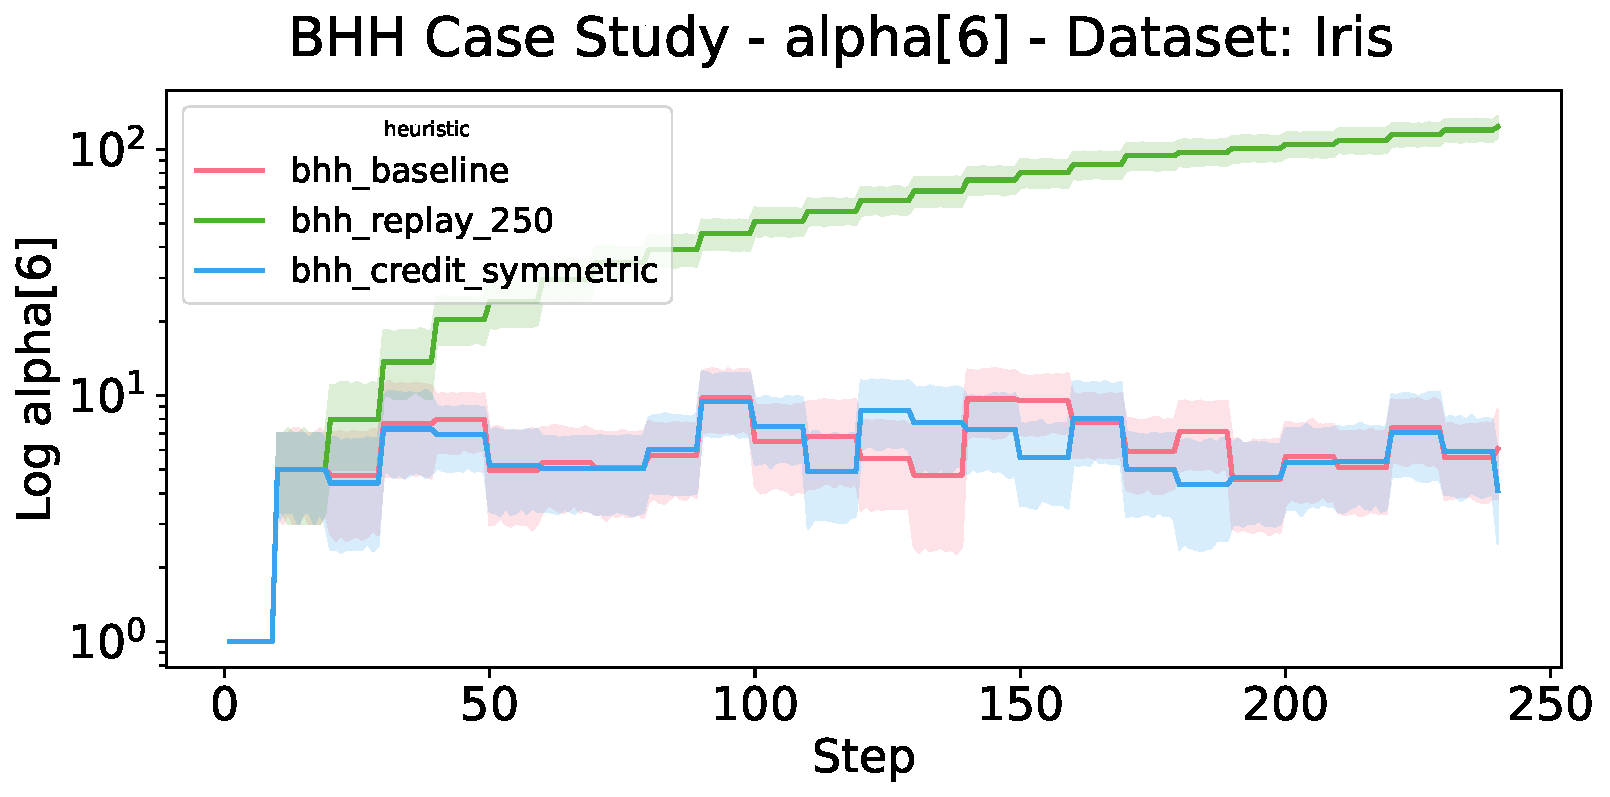
\includegraphics[width=1.0\textwidth]{case_study/params/figures/alphas/alpha[6].pdf}
	\caption{The average value of the concentration parameter $\alpha_{6}$ (\acs{Adam}) over 250 training steps, obtained from 30 runs of the case study on the behaviour of the \acs{BHH} on the Iris dataset, illustrated in log scale.}
	\label{fig:results:case_study:alpha:6}
\end{figure}

\begin{figure}[htpb]
	\centering
	\includegraphics[width=1.0\textwidth]{case_study/params/figures/alphas/alpha[7].pdf}
	\caption{The average value of the concentration parameter $\alpha_{7}$ (\acs{PSO}) over 250 training steps, obtained from 30 runs of the case study on the behaviour of the \acs{BHH} on the Iris dataset, illustrated in log scale.}
	\label{fig:results:case_study:alpha:7}
\end{figure}

\begin{figure}[htpb]
	\centering
	\includegraphics[width=1.0\textwidth]{case_study/params/figures/alphas/alpha[8].pdf}
	\caption{The average value of the concentration parameter $\alpha_{8}$ (\acs{GA}) over 250 training steps, obtained from 30 runs of the case study on the behaviour of the \acs{BHH} on the Iris dataset, illustrated in log scale.}
	\label{fig:results:case_study:alpha:8}
\end{figure}



%%%%%%%%%%%%%%%%%%%%%%%%%%%%%%%%%%%%%%%%%%%%%%%%%%%%%
% PARAMS THETAS
%%%%%%%%%%%%%%%%%%%%%%%%%%%%%%%%%%%%%%%%%%%%%%%%%%%%%

\begin{figure}[htpb]
	\centering
	\includegraphics[width=1.0\textwidth]{case_study/params/figures/thetas/theta[0].pdf}
	\caption{The average unnormalised sampled probability of the selection probability, denoted $\theta_{0}$ (\acs{SGD}), given concentration parameter $\alpha_{0}$, sampled from the probability distribution $P(\theta_{0} \vert \alpha_{0})$ over 250 steps, obtained from 30 runs of the case study on the behaviour of the \acs{BHH} on the Iris dataset, illustrated in log scale.}
	\label{fig:results:case_study:theta:0}
\end{figure}

\begin{figure}[htpb]
	\centering
	\includegraphics[width=1.0\textwidth]{case_study/params/figures/thetas/theta[6].pdf}
	\caption{The average unnormalised sampled probability of the selection probability, denoted $\theta_{6}$ (\acs{Adam}), given concentration parameter $\alpha_{6}$, sampled from the probability distribution $P(\theta_{6} \vert \alpha_{6})$ over 250 steps, obtained from 30 runs of the case study on the behaviour of the \acs{BHH} on the Iris dataset, illustrated in log scale.}
	\label{fig:results:case_study:theta:6}
\end{figure}

\begin{figure}[htpb]
	\centering
	\includegraphics[width=1.0\textwidth]{case_study/params/figures/thetas/theta[7].pdf}
	\caption{The average unnormalised sampled probability of the selection probability, denoted $\theta_{7}$ (\acs{PSO}), given concentration parameter $\alpha_{7}$, sampled from the probability distribution $P(\theta_{7} \vert \alpha_{7})$ over 250 steps, obtained from 30 runs of the case study on the behaviour of the \acs{BHH} on the Iris dataset, illustrated in log scale.}
	\label{fig:results:case_study:theta:7}
\end{figure}

\begin{figure}[htpb]
	\centering
	\includegraphics[width=1.0\textwidth]{case_study/params/figures/thetas/theta[8].pdf}
	\caption{The average unnormalised sampled probability of the selection probability, denoted $\theta_{8}$ (\acs{GA}), given concentration parameter $\alpha_{8}$, sampled from the probability distribution $P(\theta_{8} \vert \alpha_{8})$ over 250 steps, obtained from 30 runs of the case study on the behaviour of the \acs{BHH} on the Iris dataset, illustrated in log scale.}
	\label{fig:results:case_study:theta:8}
\end{figure}

%%%%%%%%%%%%%%%%%%%%%%%%%%%%%%%%%%%%%%%%%%%%%%%%%%%%%
% PARAMS P_H (Priors)
%%%%%%%%%%%%%%%%%%%%%%%%%%%%%%%%%%%%%%%%%%%%%%%%%%%%%

\begin{figure}[htpb]
	\centering
	\includegraphics[width=1.0\textwidth]{case_study/params/figures/p_H/p_H[0].pdf}
	\caption{The average unnormalised sampled prior selection probability for \index{heuristic}heuristic $h_{0}$ (\acs{SGD}), given the probability of the selection probability, denoted by $\theta_{0}$, sampled from the prior selection probability distribution $P(h_{0} \vert \theta_{0})$ over 250 steps, obtained from 30 runs of the case study on the behaviour of the \acs{BHH} on the Iris dataset, illustrated in log scale.}
	\label{fig:results:case_study:p_H:0}
\end{figure}

\begin{figure}[htpb]
	\centering
	\includegraphics[width=1.0\textwidth]{case_study/params/figures/p_H/p_H[6].pdf}
	\caption{The average unnormalised sampled prior selection probability for \index{heuristic}heuristic $h_{6}$ (\acs{Adam}), given the probability of the selection probability, denoted by $\theta_{6}$, sampled from the prior selection probability distribution $P(h_{6} \vert \theta_{6})$ over 250 steps, obtained from 30 runs of the case study on the behaviour of the \acs{BHH} on the Iris dataset, illustrated in log scale.}
	\label{fig:results:case_study:p_H:6}
\end{figure}

\begin{figure}[htpb]
	\centering
	\includegraphics[width=1.0\textwidth]{case_study/params/figures/p_H/p_H[7].pdf}
	\caption{The average unnormalised sampled prior selection probability for \index{heuristic}heuristic $h_{7}$ (\acs{PSO}), given the probability of the selection probability, denoted by $\theta_{7}$, sampled from the prior selection probability distribution $P(h_{7} \vert \theta_{7})$ over 250 steps, obtained from 30 runs of the case study on the behaviour of the \acs{BHH} on the Iris dataset, illustrated in log scale.}
	\label{fig:results:case_study:p_H:7}
\end{figure}

\begin{figure}[htpb]
	\centering
	\includegraphics[width=1.0\textwidth]{case_study/params/figures/p_H/p_H[8].pdf}
	\caption{The average unnormalised sampled prior selection probability for \index{heuristic}heuristic $h_{8}$ (\acs{GA}), given the probability of the selection probability, denoted by $\theta_{8}$, sampled from the prior selection probability distribution $P(h_{8} \vert \theta_{8})$ over 250 steps, obtained from 30 runs of the case study on the behaviour of the \acs{BHH} on the Iris dataset, illustrated in log scale.}
	\label{fig:results:case_study:p_H:8}
\end{figure}
%%%%%%%%%%%%%%%%%%%%%%%%%%%%%%%%%%%%%%%%%%%%%%%%%%%%%
% PARAMS P_HgEC (Posterior)
%%%%%%%%%%%%%%%%%%%%%%%%%%%%%%%%%%%%%%%%%%%%%%%%%%%%%

\begin{figure}[htpb]
	\centering
	\includegraphics[width=1.0\textwidth]{case_study/params/figures/p_HgEC/p_HgEC[0][0].pdf}
	\caption{The average unnormalised sampled posterior selection probability for \index{heuristic}heuristic $h_{0}$ (\acs{SGD}), given the application to entity $e_{0}$ and requiring a successful credit allocation ($\gamma_{1}$) from the \textit{ibest} credit assignment strategy, sampled from the posterior selection probability distribution $P(h_{0} \vert \theta_{0} \vert e_{0}, \gamma_{1})$ over 250 steps, obtained from 30 runs of the case study on the behaviour of the \acs{BHH} on the Iris dataset, illustrated in log scale.}
	\label{fig:results:case_study:p_HgEC:0:0}
\end{figure}


\begin{figure}[htpb]
	\centering
	\includegraphics[width=1.0\textwidth]{case_study/params/figures/p_HgEC/p_HgEC[0][6].pdf}
	\caption{The average unnormalised sampled posterior selection probability for \index{heuristic}heuristic $h_{6}$ (\acs{Adam}), given the application to entity $e_{0}$ and requiring a successful credit allocation ($\gamma_{1}$) from the \textit{ibest} credit assignment strategy, sampled from the posterior selection probability distribution $P(h_{6} \vert \theta_{6} \vert e_{0}, \gamma_{1})$ over 250 steps, obtained from 30 runs of the case study on the behaviour of the \acs{BHH} on the Iris dataset, illustrated in log scale.}
	\label{fig:results:case_study:p_HgEC:0:6}
\end{figure}

\begin{figure}[htpb]
	\centering
	\includegraphics[width=1.0\textwidth]{case_study/params/figures/p_HgEC/p_HgEC[0][7].pdf}
	\caption{The average unnormalised sampled posterior selection probability for \index{heuristic}heuristic $h_{7}$ (\acs{PSO}), given the application to entity $e_{0}$ and requiring a successful credit allocation ($\gamma_{1}$) from the \textit{ibest} credit assignment strategy, sampled from the posterior selection probability distribution $P(h_{7} \vert \theta_{7} \vert e_{0}, \gamma_{1})$ over 250 steps, obtained from 30 runs of the case study on the behaviour of the \acs{BHH} on the Iris dataset, illustrated in log scale.}
	\label{fig:results:case_study:p_HgEC:0:7}
\end{figure}

\begin{figure}[htpb]
	\centering
	\includegraphics[width=1.0\textwidth]{case_study/params/figures/p_HgEC/p_HgEC[0][8].pdf}
	\caption{The average unnormalised sampled posterior selection probability for \index{heuristic}heuristic $h_{8}$ (\acs{GA}), given the application to entity $e_{0}$ and requiring a successful credit allocation ($\gamma_{1}$) from the \textit{ibest} credit assignment strategy, sampled from the posterior selection probability distribution $P(h_{8} \vert \theta_{8} \vert e_{0}, \gamma_{1})$ over 250 steps, obtained from 30 runs of the case study on the behaviour of the \acs{BHH} on the Iris dataset, illustrated in log scale.}
	\label{fig:results:case_study:p_HgEC:0:8}
\end{figure}

\section{BHH vs. Low-Level Heuristics}\label{sec:results:bhh_vs_low_level_heuristics}

% Table generated by Excel2LaTeX from sheet 'results - test - loss'
\begin{table}[htbp]
	\centering
	\caption{Empirical results showcasing average test loss and statistics for different low-level \index{heuristic}heuristics compared to 3 \index{heuristic pool}heuristic pool variants of the baseline \acs{BHH} across multiple datasets, for all runs, at the last epoch.}
	\label{tab:results:standalone:metrics:test_loss}%
	\par\bigskip
	\resizebox{\textwidth}{!}{
		\begin{tabular}{rlccc|c|c|c|c|c|ccccc}
			epoch                                                                          & 30                 &                                                                                &                                                                                & \multicolumn{1}{r}{}                                                           & \multicolumn{1}{r}{}                            & \multicolumn{1}{r}{}                                                           & \multicolumn{1}{r}{}                            & \multicolumn{1}{r}{}                                                           & \multicolumn{1}{r}{}                            &                                                 &                                                 &                                                 &                                                 &                                                 \\
			                                                                               &                    &                                                                                &                                                                                & \multicolumn{1}{r}{}                                                           & \multicolumn{1}{r}{}                            & \multicolumn{1}{r}{}                                                           & \multicolumn{1}{r}{}                            & \multicolumn{1}{r}{}                                                           & \multicolumn{1}{r}{}                            &                                                 &                                                 &                                                 &                                                 &                                                 \\
			                                                                               &                    & \multicolumn{1}{l}{\textbf{heuristic}}                                         &                                                                                & \multicolumn{1}{r}{}                                                           & \multicolumn{1}{r}{}                            & \multicolumn{1}{r}{}                                                           & \multicolumn{1}{r}{}                            & \multicolumn{1}{r}{}                                                           & \multicolumn{1}{r}{}                            &                                                 &                                                 &                                                 &                                                 &                                                 \\
			\cmidrule{3-3}\cmidrule{6-6}\cmidrule{8-8}\cmidrule{10-10}    \textbf{dataset} & \textbf{statistic} & \textbf{adagrad}                                                               & \textbf{adam}                                                                  & \textbf{nag}                                                                   & \textbf{bhh\_gd}                                & \textbf{rmsprop}                                                               & \textbf{bhh\_all}                               & \textbf{adadelta}                                                              & \textbf{bhh\_mh}                                & \textbf{ga}                                     & \textbf{sgd}                                    & \textbf{pso}                                    & \textbf{momentum}                               & \textbf{de}                                     \\
			\midrule
			abalone                                                                        & count              & 30                                                                             & 30                                                                             & 30                                                                             & 30                                              & 30                                                                             & 30                                              & 30                                                                             & 30                                              & 30                                              & 30                                              & 30                                              & 30                                              & 30                                              \\
			                                                                               & avg                & \cellcolor[rgb]{ .506,  .776,  .486}1.967785                                   & \cellcolor[rgb]{ .494,  .773,  .486}1.965134827                                & \cellcolor[rgb]{ .765,  .851,  .502}2.0156043                                  & \cellcolor[rgb]{ .749,  .847,  .502}2.012517173 & \cellcolor[rgb]{ .388,  .745,  .482}\textcolor[rgb]{ 0,  .38,  0}{1.94553315}  & \cellcolor[rgb]{ 1,  .922,  .518}2.058704583    & \cellcolor[rgb]{ .788,  .859,  .502}2.019921077                                & \cellcolor[rgb]{ .996,  .827,  .502}2.29420573  & \cellcolor[rgb]{ .984,  .612,  .459}2.81545685  & \cellcolor[rgb]{ .992,  .773,  .49}2.42804241   & \cellcolor[rgb]{ .98,  .522,  .443}3.038417873  & \cellcolor[rgb]{ .992,  .745,  .486}2.494169393 & \cellcolor[rgb]{ .973,  .412,  .42}3.295858177  \\
			                                                                               & std                & 0.031577789                                                                    & 0.034949967                                                                    & 0.034657443                                                                    & 0.068121366                                     & 0.035183664                                                                    & 0.087594488                                     & 0.034405331                                                                    & 0.055085207                                     & 0.055148148                                     & 0.028810924                                     & 0.293755503                                     & 0.029086341                                     & 0.016489872                                     \\
			adult                                                                          & count              & 30                                                                             & 30                                                                             & 30                                                                             & 30                                              & 30                                                                             & 30                                              & 30                                                                             & 30                                              & 30                                              & 30                                              & 30                                              & 30                                              & 30                                              \\
			                                                                               & avg                & \cellcolor[rgb]{ 1,  .922,  .518}0.346737798                                   & \cellcolor[rgb]{ 1,  .922,  .518}0.38233353                                    & \cellcolor[rgb]{ .388,  .745,  .482}\textcolor[rgb]{ 0,  .38,  0}{0.313320884} & \cellcolor[rgb]{ .788,  .859,  .502}0.335180995 & \cellcolor[rgb]{ .933,  .902,  .514}0.343292783                                & \cellcolor[rgb]{ .973,  .412,  .42}586.2065996  & \cellcolor[rgb]{ .467,  .765,  .486}0.317677033                                & \cellcolor[rgb]{ 1,  .922,  .518}0.363543899    & \cellcolor[rgb]{ 1,  .922,  .518}0.392047161    & \cellcolor[rgb]{ .388,  .745,  .482}0.313329677 & \cellcolor[rgb]{ 1,  .922,  .518}1.217724345    & \cellcolor[rgb]{ .388,  .745,  .482}0.313444396 & \cellcolor[rgb]{ 1,  .922,  .518}0.639695856    \\
			                                                                               & std                & 0.003704238                                                                    & 0.018067239                                                                    & 0.000510377                                                                    & 0.043628962                                     & 0.014659665                                                                    & 1261.204704                                     & 0.005277776                                                                    & 0.020803371                                     & 0.020086997                                     & 0.000411017                                     & 0.496591684                                     & 0.0003947                                       & 0.042558869                                     \\
			air quality                                                                    & count              & 30                                                                             & 30                                                                             & 30                                                                             & 30                                              & 30                                                                             & 30                                              & 30                                                                             & 30                                              & 30                                              & 30                                              & 30                                              & 30                                              & 30                                              \\
			                                                                               & avg                & \cellcolor[rgb]{ .651,  .82,  .494}0.256871193                                 & \cellcolor[rgb]{ .827,  .871,  .506}0.260623969                                & \cellcolor[rgb]{ .647,  .82,  .494}0.256829053                                 & \cellcolor[rgb]{ 1,  .922,  .518}0.264177871    & \cellcolor[rgb]{ .388,  .745,  .482}\textcolor[rgb]{ 0,  .38,  0}{0.251334045} & \cellcolor[rgb]{ .996,  .827,  .502}0.272859303 & \cellcolor[rgb]{ .647,  .82,  .494}0.256781683                                 & \cellcolor[rgb]{ .976,  .914,  .514}0.263703859 & \cellcolor[rgb]{ .996,  .792,  .494}0.275862527 & \cellcolor[rgb]{ .988,  .69,  .475}0.285172782  & \cellcolor[rgb]{ .984,  .608,  .459}0.292264593 & \cellcolor[rgb]{ .984,  .604,  .459}0.292851261 & \cellcolor[rgb]{ .973,  .412,  .42}0.309698115  \\
			                                                                               & std                & 0.007475522                                                                    & 0.008912099                                                                    & 0.005955119                                                                    & 0.011452365                                     & 0.007814891                                                                    & 0.016310047                                     & 0.00630808                                                                     & 0.007306605                                     & 0.008162884                                     & 0.014769128                                     & 0.022648597                                     & 0.016417541                                     & 0.017044223                                     \\
			bank                                                                           & count              & 30                                                                             & 30                                                                             & 30                                                                             & 30                                              & 30                                                                             & 30                                              & 30                                                                             & 30                                              & 30                                              & 30                                              & 30                                              & 30                                              & 30                                              \\
			                                                                               & avg                & \cellcolor[rgb]{ .459,  .765,  .486}0.209641222                                & \cellcolor[rgb]{ .4,  .745,  .482}0.206461621                                  & \cellcolor[rgb]{ .588,  .8,  .49}0.2164275                                     & \cellcolor[rgb]{ .588,  .8,  .49}0.21643132     & \cellcolor[rgb]{ .388,  .745,  .482}\textcolor[rgb]{ 0,  .38,  0}{0.205779476} & \cellcolor[rgb]{ 1,  .886,  .514}0.245610465    & \cellcolor[rgb]{ .627,  .812,  .494}0.218599386                                & \cellcolor[rgb]{ .996,  .839,  .502}0.256171151 & \cellcolor[rgb]{ .988,  .686,  .475}0.28813827  & \cellcolor[rgb]{ 1,  .922,  .518}0.238179998    & \cellcolor[rgb]{ .973,  .412,  .42}0.345448185  & \cellcolor[rgb]{ 1,  .922,  .518}0.238550439    & \cellcolor[rgb]{ .976,  .424,  .424}0.343699166 \\
			                                                                               & std                & 0.004750498                                                                    & 0.004040969                                                                    & 0.005944898                                                                    & 0.004889433                                     & 0.005654034                                                                    & 0.064531685                                     & 0.003821749                                                                    & 0.010550504                                     & 0.012801143                                     & 0.005568018                                     & 0.033990143                                     & 0.004820977                                     & 0.028120079                                     \\
			bike                                                                           & count              & 30                                                                             & 30                                                                             & 30                                                                             & 30                                              & 30                                                                             & 30                                              & 30                                                                             & 30                                              & 30                                              & 30                                              & 30                                              & 30                                              & 30                                              \\
			                                                                               & avg                & \cellcolor[rgb]{ .388,  .745,  .482}\textcolor[rgb]{ 0,  .38,  0}{0.045805387} & \cellcolor[rgb]{ .592,  .804,  .494}0.068179412                                & \cellcolor[rgb]{ .882,  .886,  .51}0.099539486                                 & \cellcolor[rgb]{ .467,  .765,  .486}0.054496914 & \cellcolor[rgb]{ 1,  .922,  .518}0.112259627                                   & \cellcolor[rgb]{ .565,  .796,  .49}0.065136647  & \cellcolor[rgb]{ .588,  .8,  .49}0.06793708                                    & \cellcolor[rgb]{ 1,  .902,  .514}0.11787523     & \cellcolor[rgb]{ .992,  .761,  .486}0.153095534 & \cellcolor[rgb]{ .992,  .733,  .482}0.159868436 & \cellcolor[rgb]{ .992,  .773,  .49}0.150273084  & \cellcolor[rgb]{ .992,  .725,  .482}0.161397393 & \cellcolor[rgb]{ .973,  .412,  .42}0.239867227  \\
			                                                                               & std                & 0.001725608                                                                    & 0.068117237                                                                    & 0.001754469                                                                    & 0.005239285                                     & 0.103490928                                                                    & 0.019626763                                     & 0.002076596                                                                    & 0.005954748                                     & 0.005079692                                     & 0.002759                                        & 0.025177188                                     & 0.003354245                                     & 0.039791214                                     \\
			car                                                                            & count              & 30                                                                             & 30                                                                             & 30                                                                             & 30                                              & 30                                                                             & 30                                              & 30                                                                             & 30                                              & 30                                              & 30                                              & 30                                              & 30                                              & 30                                              \\
			                                                                               & avg                & \cellcolor[rgb]{ .729,  .843,  .502}0.202726327                                & \cellcolor[rgb]{ .388,  .745,  .482}\textcolor[rgb]{ 0,  .38,  0}{0.09724452}  & \cellcolor[rgb]{ .867,  .882,  .51}0.245363623                                 & \cellcolor[rgb]{ .62,  .812,  .494}0.16895294   & \cellcolor[rgb]{ .408,  .749,  .482}0.103937737                                & \cellcolor[rgb]{ .58,  .8,  .49}0.15718728      & \cellcolor[rgb]{ 1,  .922,  .518}0.285888989                                   & \cellcolor[rgb]{ .992,  .733,  .482}0.489062582 & \cellcolor[rgb]{ .98,  .502,  .439}0.737354357  & \cellcolor[rgb]{ .98,  .533,  .443}0.703539757  & \cellcolor[rgb]{ .988,  .667,  .471}0.563173207 & \cellcolor[rgb]{ .98,  .506,  .439}0.73217904   & \cellcolor[rgb]{ .973,  .412,  .42}0.833160108  \\
			                                                                               & std                & 0.018356416                                                                    & 0.023870777                                                                    & 0.028744869                                                                    & 0.025441117                                     & 0.031133074                                                                    & 0.033710554                                     & 0.027353972                                                                    & 0.076505599                                     & 0.062600847                                     & 0.052091474                                     & 0.157928484                                     & 0.042705727                                     & 0.074182791                                     \\
			diabetic                                                                       & count              & 30                                                                             & 30                                                                             & 30                                                                             & 30                                              & 30                                                                             & 30                                              & 30                                                                             & 30                                              & 30                                              & 30                                              & 30                                              & 30                                              & 30                                              \\
			                                                                               & avg                & \cellcolor[rgb]{ .694,  .831,  .498}0.889537739                                & \cellcolor[rgb]{ 1,  .898,  .514}0.919339482                                   & \cellcolor[rgb]{ .388,  .745,  .482}\textcolor[rgb]{ 0,  .38,  0}{0.880898965} & \cellcolor[rgb]{ .98,  .914,  .514}0.897587026  & \cellcolor[rgb]{ .918,  .894,  .51}0.895749019                                 & \cellcolor[rgb]{ .973,  .412,  .42}1.298319185  & \cellcolor[rgb]{ .49,  .773,  .486}0.883864405                                 & \cellcolor[rgb]{ 1,  .902,  .518}0.913694494    & \cellcolor[rgb]{ .996,  .843,  .506}0.961291775 & \cellcolor[rgb]{ .976,  .914,  .514}0.897429714 & \cellcolor[rgb]{ .996,  .835,  .502}0.966103049 & \cellcolor[rgb]{ 1,  .922,  .518}0.898038783    & \cellcolor[rgb]{ .988,  .694,  .475}1.077362637 \\
			                                                                               & std                & 0.004272255                                                                    & 0.00981794                                                                     & 0.003758597                                                                    & 0.010748722                                     & 0.004045488                                                                    & 0.659754133                                     & 0.004759234                                                                    & 0.008388702                                     & 0.00657199                                      & 0.003551413                                     & 0.016450474                                     & 0.002801135                                     & 0.0391395                                       \\
			fish toxicity                                                                  & count              & 30                                                                             & 30                                                                             & 30                                                                             & 30                                              & 30                                                                             & 30                                              & 30                                                                             & 30                                              & 30                                              & 30                                              & 30                                              & 30                                              & 30                                              \\
			                                                                               & avg                & \cellcolor[rgb]{ .588,  .8,  .49}0.09908239                                    & \cellcolor[rgb]{ .451,  .761,  .482}0.097196901                                & \cellcolor[rgb]{ .831,  .871,  .506}0.10233624                                 & \cellcolor[rgb]{ 1,  .91,  .518}0.105584544     & \cellcolor[rgb]{ .388,  .745,  .482}\textcolor[rgb]{ 0,  .38,  0}{0.096326802} & \cellcolor[rgb]{ 1,  .922,  .518}0.104598099    & \cellcolor[rgb]{ .773,  .855,  .502}0.101567158                                & \cellcolor[rgb]{ .976,  .914,  .514}0.104293618 & \cellcolor[rgb]{ 1,  .863,  .506}0.109342435    & \cellcolor[rgb]{ .976,  .475,  .435}0.139280655 & \cellcolor[rgb]{ 1,  .855,  .506}0.109946059    & \cellcolor[rgb]{ .973,  .412,  .42}0.144088336  & \cellcolor[rgb]{ .992,  .733,  .482}0.119344204 \\
			                                                                               & std                & 0.008463336                                                                    & 0.006948088                                                                    & 0.007611236                                                                    & 0.008228438                                     & 0.008021585                                                                    & 0.008136956                                     & 0.008882708                                                                    & 0.00895412                                      & 0.008990894                                     & 0.012326524                                     & 0.012481736                                     & 0.012407706                                     & 0.0130782                                       \\
			forest fires                                                                   & count              & 30                                                                             & 30                                                                             & 30                                                                             & 30                                              & 30                                                                             & 30                                              & 30                                                                             & 30                                              & 30                                              & 30                                              & 30                                              & 30                                              & 30                                              \\
			                                                                               & avg                & \cellcolor[rgb]{ 1,  .922,  .518}0.064321917                                   & \cellcolor[rgb]{ .557,  .792,  .49}0.052658676                                 & \cellcolor[rgb]{ .851,  .878,  .506}0.05923886                                 & \cellcolor[rgb]{ .824,  .871,  .506}0.058617148 & \cellcolor[rgb]{ 1,  .922,  .518}0.062552555                                   & \cellcolor[rgb]{ 1,  .89,  .514}0.080966845     & \cellcolor[rgb]{ .388,  .745,  .482}\textcolor[rgb]{ 0,  .38,  0}{0.048831474} & \cellcolor[rgb]{ .976,  .914,  .514}0.06209696  & \cellcolor[rgb]{ .553,  .792,  .49}0.05260701   & \cellcolor[rgb]{ .992,  .722,  .482}0.180571383 & \cellcolor[rgb]{ 1,  .914,  .518}0.069210426    & \cellcolor[rgb]{ .992,  .706,  .478}0.188476672 & \cellcolor[rgb]{ .973,  .412,  .42}0.359831599  \\
			                                                                               & std                & 0.039911806                                                                    & 0.039243672                                                                    & 0.031685801                                                                    & 0.034163415                                     & 0.039170629                                                                    & 0.069099845                                     & 0.032095867                                                                    & 0.038470671                                     & 0.025957821                                     & 0.008365929                                     & 0.047244856                                     & 0.010081381                                     & 0.089999905                                     \\
			housing                                                                        & count              & 30                                                                             & 30                                                                             & 30                                                                             & 30                                              & 30                                                                             & 30                                              & 30                                                                             & 30                                              & 30                                              & 30                                              & 30                                              & 30                                              & 30                                              \\
			                                                                               & avg                & \cellcolor[rgb]{ .518,  .78,  .486}0.088925893                                 & \cellcolor[rgb]{ .404,  .749,  .482}0.08481865                                 & \cellcolor[rgb]{ .612,  .808,  .494}0.092269667                                & \cellcolor[rgb]{ .69,  .831,  .498}0.095072459  & \cellcolor[rgb]{ .388,  .745,  .482}\textcolor[rgb]{ 0,  .38,  0}{0.08422333}  & \cellcolor[rgb]{ .663,  .824,  .498}0.094078934 & \cellcolor[rgb]{ 1,  .922,  .518}0.105999965                                   & \cellcolor[rgb]{ 1,  .867,  .51}0.116883814     & \cellcolor[rgb]{ .996,  .812,  .498}0.127851649 & \cellcolor[rgb]{ .984,  .576,  .455}0.173521216 & \cellcolor[rgb]{ .992,  .722,  .482}0.145240159 & \cellcolor[rgb]{ .984,  .588,  .455}0.171302372 & \cellcolor[rgb]{ .973,  .412,  .42}0.205724786  \\
			                                                                               & std                & 0.012490666                                                                    & 0.011213172                                                                    & 0.015551947                                                                    & 0.014823695                                     & 0.014924594                                                                    & 0.017302471                                     & 0.018700331                                                                    & 0.019460369                                     & 0.020192262                                     & 0.022837541                                     & 0.029813905                                     & 0.017916976                                     & 0.036445189                                     \\
			iris                                                                           & count              & 30                                                                             & 30                                                                             & 30                                                                             & 30                                              & 30                                                                             & 30                                              & 30                                                                             & 30                                              & 30                                              & 30                                              & 30                                              & 30                                              & 30                                              \\
			                                                                               & avg                & \cellcolor[rgb]{ .788,  .859,  .502}0.216138929                                & \cellcolor[rgb]{ .514,  .78,  .486}0.120305813                                 & \cellcolor[rgb]{ .416,  .753,  .482}0.084967127                                & \cellcolor[rgb]{ 1,  .855,  .506}0.372908547    & \cellcolor[rgb]{ .388,  .745,  .482}\textcolor[rgb]{ 0,  .38,  0}{0.075287772} & \cellcolor[rgb]{ .859,  .878,  .506}0.241094806 & \cellcolor[rgb]{ .996,  .808,  .498}0.426015649                                & \cellcolor[rgb]{ .686,  .831,  .498}0.180917533 & \cellcolor[rgb]{ 1,  .922,  .518}0.289495446    & \cellcolor[rgb]{ .992,  .773,  .49}0.469415404  & \cellcolor[rgb]{ .973,  .412,  .42}0.896458149  & \cellcolor[rgb]{ .992,  .745,  .486}0.502796506 & \cellcolor[rgb]{ .98,  .494,  .435}0.802733988  \\
			                                                                               & std                & 0.059156887                                                                    & 0.097731271                                                                    & 0.041820159                                                                    & 1.119111663                                     & 0.045657899                                                                    & 0.295227964                                     & 0.071608458                                                                    & 0.163729792                                     & 0.117435582                                     & 0.087556703                                     & 0.844445785                                     & 0.072001841                                     & 0.684394699                                     \\
			mushroom                                                                       & count              & 30                                                                             & 30                                                                             & 30                                                                             & 30                                              & 30                                                                             & 30                                              & 30                                                                             & 30                                              & 30                                              & 30                                              & 30                                              & 30                                              & 30                                              \\
			                                                                               & avg                & \cellcolor[rgb]{ .549,  .792,  .49}0.002577835                                 & \cellcolor[rgb]{ .467,  .765,  .486}0.001321295                                & \cellcolor[rgb]{ 1,  .922,  .518}0.009417256                                   & \cellcolor[rgb]{ .439,  .757,  .482}0.000906998 & \cellcolor[rgb]{ .388,  .745,  .482}\textcolor[rgb]{ 0,  .38,  0}{8.30695E-05} & \cellcolor[rgb]{ .718,  .839,  .498}0.005152476 & \cellcolor[rgb]{ .655,  .82,  .494}0.00417499                                  & \cellcolor[rgb]{ 1,  .871,  .51}0.077415858     & \cellcolor[rgb]{ .984,  .561,  .451}0.489160105 & \cellcolor[rgb]{ .996,  .796,  .494}0.179705445 & \cellcolor[rgb]{ 1,  .886,  .514}0.061137885    & \cellcolor[rgb]{ .992,  .749,  .486}0.241811308 & \cellcolor[rgb]{ .973,  .412,  .42}0.687017333  \\
			                                                                               & std                & 0.000662841                                                                    & 0.004905902                                                                    & 0.002279151                                                                    & 0.001259819                                     & 6.96496E-05                                                                    & 0.012039998                                     & 0.000905097                                                                    & 0.019865901                                     & 0.024593143                                     & 0.009208458                                     & 0.06033175                                      & 0.012790223                                     & 0.01638976                                      \\
			parkinsons                                                                     & count              & 30                                                                             & 30                                                                             & 30                                                                             & 30                                              & 30                                                                             & 30                                              & 30                                                                             & 30                                              & 30                                              & 30                                              & 30                                              & 30                                              & 30                                              \\
			                                                                               & avg                & \cellcolor[rgb]{ .51,  .776,  .486}0.056277858                                 & \cellcolor[rgb]{ .412,  .749,  .482}0.054480758                                & \cellcolor[rgb]{ 1,  .922,  .518}0.065451464                                   & \cellcolor[rgb]{ .639,  .816,  .494}0.058737776 & \cellcolor[rgb]{ .388,  .745,  .482}\textcolor[rgb]{ 0,  .38,  0}{0.053985977} & \cellcolor[rgb]{ .639,  .816,  .494}0.05873821  & \cellcolor[rgb]{ .69,  .831,  .498}0.05967759                                  & \cellcolor[rgb]{ 1,  .918,  .518}0.065774264    & \cellcolor[rgb]{ 1,  .898,  .514}0.066854953    & \cellcolor[rgb]{ .976,  .467,  .431}0.092323864 & \cellcolor[rgb]{ 1,  .894,  .514}0.067066667    & \cellcolor[rgb]{ .973,  .412,  .42}0.095371925  & \cellcolor[rgb]{ .984,  .604,  .459}0.084321583 \\
			                                                                               & std                & 0.001432862                                                                    & 0.001998668                                                                    & 0.002301839                                                                    & 0.002859752                                     & 0.001547989                                                                    & 0.002811075                                     & 0.001691389                                                                    & 0.002548177                                     & 0.003281185                                     & 0.008302374                                     & 0.005043049                                     & 0.009431099                                     & 0.008978517                                     \\
			student performance                                                            & count              & 30                                                                             & 30                                                                             & 30                                                                             & 30                                              & 30                                                                             & 30                                              & 30                                                                             & 30                                              & 30                                              & 30                                              & 30                                              & 30                                              & 30                                              \\
			                                                                               & avg                & \cellcolor[rgb]{ .388,  .745,  .482}\textcolor[rgb]{ 0,  .38,  0}{0.165552792} & \cellcolor[rgb]{ .98,  .522,  .443}0.492891063                                 & \cellcolor[rgb]{ .471,  .769,  .486}0.169715979                                & \cellcolor[rgb]{ 1,  .855,  .506}0.245419875    & \cellcolor[rgb]{ .973,  .412,  .42}0.572439541                                 & \cellcolor[rgb]{ 1,  .871,  .51}0.235942235     & \cellcolor[rgb]{ .49,  .773,  .486}0.170794263                                 & \cellcolor[rgb]{ .969,  .91,  .514}0.194664435  & \cellcolor[rgb]{ 1,  .922,  .518}0.196187948    & \cellcolor[rgb]{ .933,  .902,  .514}0.193041307 & \cellcolor[rgb]{ .984,  .573,  .451}0.456490052 & \cellcolor[rgb]{ .925,  .898,  .51}0.192542094  & \cellcolor[rgb]{ 1,  .918,  .518}0.201390878    \\
			                                                                               & std                & 0.011258528                                                                    & 0.105388532                                                                    & 0.010966961                                                                    & 0.133694251                                     & 0.05360667                                                                     & 0.10249181                                      & 0.010377173                                                                    & 0.014024256                                     & 0.009798773                                     & 0.011295962                                     & 0.049033016                                     & 0.011402763                                     & 0.011757846                                     \\
			wine quality                                                                   & count              & 30                                                                             & 30                                                                             & 30                                                                             & 30                                              & 30                                                                             & 30                                              & 30                                                                             & 30                                              & 30                                              & 30                                              & 30                                              & 30                                              & 30                                              \\
			                                                                               & avg                & \cellcolor[rgb]{ .631,  .816,  .494}1.06505343                                 & \cellcolor[rgb]{ .388,  .745,  .482}\textcolor[rgb]{ 0,  .38,  0}{1.039511785} & \cellcolor[rgb]{ .698,  .831,  .498}1.07178488                                 & \cellcolor[rgb]{ 1,  .922,  .518}1.102805083    & \cellcolor[rgb]{ .502,  .776,  .486}1.051442793                                & \cellcolor[rgb]{ .804,  .863,  .506}1.082728853 & \cellcolor[rgb]{ .788,  .859,  .502}1.080905303                                & \cellcolor[rgb]{ .996,  .839,  .502}1.166586247 & \cellcolor[rgb]{ .992,  .725,  .482}1.251597837 & \cellcolor[rgb]{ .996,  .843,  .502}1.16477848  & \cellcolor[rgb]{ .988,  .659,  .467}1.3045869   & \cellcolor[rgb]{ .996,  .824,  .502}1.17741444  & \cellcolor[rgb]{ .973,  .412,  .42}1.489554557  \\
			                                                                               & std                & 0.023560192                                                                    & 0.018361143                                                                    & 0.024922811                                                                    & 0.039250798                                     & 0.020795097                                                                    & 0.026483778                                     & 0.021109916                                                                    & 0.030251195                                     & 0.045716819                                     & 0.022984412                                     & 0.114260845                                     & 0.01919043                                      & 0.092922599                                     \\
			\bottomrule
		\end{tabular}%
	}
\end{table}%

% Table generated by Excel2LaTeX from sheet 'results - test - rank'
\begin{table}[htbp]
	\centering
	\caption{Empirical results showcasing normalised average rank and statistics for different low-level \index{heuristic}heuristics compared to 3 \index{heuristic pool}heuristic pool variants of the baseline \acs{BHH} across multiple datasets, for all runs and epochs.}
	\label{tab:results:standalone:metrics:rank}%
	\par\bigskip
	\resizebox{\textwidth}{!}{
		\begin{tabular}{rcccc|c|c|c|c|c|ccccc}
			epoch                                                                          & \multicolumn{1}{l}{(all)}              &                                                                                    &                                                                           & \multicolumn{1}{r}{}                                                      & \multicolumn{1}{r}{}                           & \multicolumn{1}{r}{}                                                      & \multicolumn{1}{r}{}                         & \multicolumn{1}{r}{}                        & \multicolumn{1}{r}{}                           &                                                &                                                 &                                                 &                                                &                                                \\
			                                                                               &                                        &                                                                                    &                                                                           & \multicolumn{1}{r}{}                                                      & \multicolumn{1}{r}{}                           & \multicolumn{1}{r}{}                                                      & \multicolumn{1}{r}{}                         & \multicolumn{1}{r}{}                        & \multicolumn{1}{r}{}                           &                                                &                                                 &                                                 &                                                &                                                \\
			                                                                               &                                        & \multicolumn{1}{l}{\textbf{heuristic}}                                             &                                                                           & \multicolumn{1}{r}{}                                                      & \multicolumn{1}{r}{}                           & \multicolumn{1}{r}{}                                                      & \multicolumn{1}{r}{}                         & \multicolumn{1}{r}{}                        & \multicolumn{1}{r}{}                           &                                                &                                                 &                                                 &                                                &                                                \\
			\cmidrule{3-3}\cmidrule{6-6}\cmidrule{8-8}\cmidrule{10-10}    \textbf{dataset} & \multicolumn{1}{l}{\textbf{statistic}} & \textbf{adagrad}                                                                   & \textbf{adam}                                                             & \textbf{nag}                                                              & \textbf{bhh\_gd}                               & \textbf{rmsprop}                                                          & \textbf{bhh\_all}                            & \textbf{adadelta}                           & \textbf{bhh\_mh}                               & \textbf{ga}                                    & \textbf{sgd}                                    & \textbf{pso}                                    & \textbf{momentum}                              & \textbf{de}                                    \\
			\midrule
			abalone                                                                        & count                                  & 930                                                                                & 930                                                                       & 930                                                                       & 930                                            & 930                                                                       & 930                                          & 930                                         & 930                                            & 930                                            & 930                                             & 930                                             & 930                                            & 930                                            \\
			                                                                               & avg                                    & \cellcolor[rgb]{ .776,  .937,  .808}\textcolor[rgb]{ 0,  .38,  0}{2.2215}          & 2.3989                                                                    & 4.2731                                                                    & 4.7032                                         & 4.6172                                                                    & 5.9376                                       & 5.3129                                      & 8.1882                                         & 11.1108                                        & 8.6280                                          & 11.2559                                         & 9.8151                                         & 12.5376                                        \\
			                                                                               & std                                    & 1.5913                                                                             & 1.8873                                                                    & 1.5419                                                                    & 2.1080                                         & 2.6504                                                                    & 2.3994                                       & 1.4782                                      & 1.1947                                         & 1.1017                                         & 1.0193                                          & 1.8265                                          & 1.1601                                         & 1.3291                                         \\
			adult                                                                          & count                                  & 930                                                                                & 930                                                                       & 930                                                                       & 930                                            & 930                                                                       & 930                                          & 930                                         & 930                                            & 930                                            & 930                                             & 930                                             & 930                                            & 930                                            \\
			                                                                               & avg                                    & 5.8978                                                                             & 7.6258                                                                    & \cellcolor[rgb]{ .776,  .937,  .808}\textcolor[rgb]{ 0,  .38,  0}{1.5140} & 5.3258                                         & 6.6892                                                                    & 12.0194                                      & 2.5258                                      & 7.9409                                         & 9.5860                                         & 3.0065                                          & 11.5344                                         & 3.8699                                         & 10.9462                                        \\
			                                                                               & std                                    & 1.6171                                                                             & 2.0293                                                                    & 0.7250                                                                    & 1.8985                                         & 1.8347                                                                    & 2.7430                                       & 1.3543                                      & 1.6391                                         & 1.7015                                         & 1.4999                                          & 2.0122                                          & 1.7090                                         & 1.8965                                         \\
			air quality                                                                    & count                                  & 930                                                                                & 930                                                                       & 930                                                                       & 930                                            & 930                                                                       & 930                                          & 930                                         & 930                                            & 930                                            & 930                                             & 930                                             & 930                                            & 930                                            \\
			                                                                               & avg                                    & 3.6409                                                                             & 5.4312                                                                    & 3.8194                                                                    & 5.0817                                         & \cellcolor[rgb]{ .776,  .937,  .808}\textcolor[rgb]{ 0,  .38,  0}{3.4452} & 6.6860                                       & 5.2441                                      & 6.3570                                         & 7.8204                                         & 10.6613                                         & 9.9151                                          & 11.7559                                        & 11.1419                                        \\
			                                                                               & std                                    & 2.2588                                                                             & 2.6198                                                                    & 2.2285                                                                    & 2.7618                                         & 2.5704                                                                    & 3.0613                                       & 3.1622                                      & 2.3031                                         & 2.2652                                         & 1.6061                                          & 2.2882                                          & 1.4730                                         & 2.2361                                         \\
			bank                                                                           & count                                  & 930                                                                                & 930                                                                       & 930                                                                       & 930                                            & 930                                                                       & 930                                          & 930                                         & 930                                            & 930                                            & 930                                             & 930                                             & 930                                            & 930                                            \\
			                                                                               & avg                                    & 2.5495                                                                             & \cellcolor[rgb]{ .776,  .937,  .808}\textcolor[rgb]{ 0,  .38,  0}{2.0796} & 4.2871                                                                    & 4.8828                                         & 3.4645                                                                    & 6.2419                                       & 5.6720                                      & 9.7495                                         & 10.9817                                        & 8.2774                                          & 11.8376                                         & 8.4774                                         & 12.4989                                        \\
			                                                                               & std                                    & 1.5980                                                                             & 1.5871                                                                    & 1.7325                                                                    & 1.7017                                         & 2.2090                                                                    & 2.1571                                       & 1.2411                                      & 1.0482                                         & 1.2165                                         & 1.0304                                          & 1.4638                                          & 1.0682                                         & 1.2243                                         \\
			bike                                                                           & count                                  & 930                                                                                & 930                                                                       & 930                                                                       & 930                                            & 930                                                                       & 930                                          & 930                                         & 930                                            & 930                                            & 930                                             & 930                                             & 930                                            & 930                                            \\
			                                                                               & avg                                    & \cellcolor[rgb]{ .776,  .937,  .808}\textcolor[rgb]{ 0,  .38,  0}{1.7204}          & 3.6925                                                                    & 6.4516                                                                    & 3.8441                                         & 6.2624                                                                    & 4.2151                                       & 5.3602                                      & 7.4108                                         & 9.2269                                         & 10.3355                                         & 9.3086                                          & 10.7086                                        & 12.4634                                        \\
			                                                                               & std                                    & 1.3839                                                                             & 4.0038                                                                    & 1.0199                                                                    & 1.3983                                         & 4.5803                                                                    & 1.3611                                       & 1.1555                                      & 1.0076                                         & 1.1835                                         & 1.4193                                          & 1.7615                                          & 1.4233                                         & 1.4648                                         \\
			car                                                                            & count                                  & 930                                                                                & 930                                                                       & 930                                                                       & 930                                            & 930                                                                       & 930                                          & 930                                         & 930                                            & 930                                            & 930                                             & 930                                             & 930                                            & 930                                            \\
			                                                                               & avg                                    & 4.7634                                                                             & \cellcolor[rgb]{ .776,  .937,  .808}\textcolor[rgb]{ 0,  .38,  0}{1.6226} & 6.0785                                                                    & 3.3473                                         & 2.3269                                                                    & 3.5624                                       & 7.7344                                      & 8.8505                                         & 10.7763                                        & 10.2452                                         & 8.3613                                          & 10.9226                                        & 12.4086                                        \\
			                                                                               & std                                    & 0.9383                                                                             & 1.4053                                                                    & 0.7991                                                                    & 1.3499                                         & 1.4091                                                                    & 1.3152                                       & 1.7464                                      & 1.4128                                         & 1.4715                                         & 1.4474                                          & 1.6222                                          & 1.3489                                         & 1.4915                                         \\
			diabetic                                                                       & count                                  & 930                                                                                & 930                                                                       & 930                                                                       & 930                                            & 930                                                                       & 930                                          & 930                                         & 930                                            & 930                                            & 930                                             & 930                                             & 930                                            & 930                                            \\
			                                                                               & avg                                    & 2.7796                                                                             & 7.1484                                                                    & \cellcolor[rgb]{ .776,  .937,  .808}\textcolor[rgb]{ 0,  .38,  0}{1.8118} & 5.2269                                         & 6.7376                                                                    & 9.3968                                       & 2.6753                                      & 8.5570                                         & 11.2011                                        & 5.9215                                          & 10.7022                                         & 6.3355                                         & 12.5065                                        \\
			                                                                               & std                                    & 1.6587                                                                             & 2.2265                                                                    & 1.4127                                                                    & 2.1860                                         & 2.5767                                                                    & 3.0221                                       & 1.6286                                      & 1.1699                                         & 1.4132                                         & 1.5421                                          & 1.0674                                          & 1.6118                                         & 1.2417                                         \\
			fish toxicity                                                                  & count                                  & 930                                                                                & 930                                                                       & 930                                                                       & 930                                            & 930                                                                       & 930                                          & 930                                         & 930                                            & 930                                            & 930                                             & 930                                             & 930                                            & 930                                            \\
			                                                                               & avg                                    & 4.2645                                                                             & 3.6022                                                                    & 5.8914                                                                    & 5.4118                                         & \cellcolor[rgb]{ .776,  .937,  .808}\textcolor[rgb]{ 0,  .38,  0}{3.5946} & 5.8290                                       & 7.9140                                      & 6.3849                                         & 6.7043                                         & 11.5785                                         & 7.5731                                          & 12.2301                                        & 10.0215                                        \\
			                                                                               & std                                    & 2.6142                                                                             & 2.4453                                                                    & 2.6288                                                                    & 2.6649                                         & 2.3292                                                                    & 2.8557                                       & 3.4287                                      & 2.9437                                         & 2.8200                                         & 1.4587                                          & 2.9817                                          & 1.3822                                         & 2.3585                                         \\
			forest fires                                                                   & count                                  & 930                                                                                & 930                                                                       & 930                                                                       & 930                                            & 930                                                                       & 930                                          & 930                                         & 930                                            & 930                                            & 930                                             & 930                                             & 930                                            & 930                                            \\
			                                                                               & avg                                    & 5.1559                                                                             & \cellcolor[rgb]{ .776,  .937,  .808}\textcolor[rgb]{ 0,  .38,  0}{4.2688} & 5.6882                                                                    & 4.6935                                         & 5.0355                                                                    & 5.4839                                       & 6.5161                                      & 5.4591                                         & 7.3667                                         & 10.8129                                         & 6.4796                                          & 11.7065                                        & 12.3333                                        \\
			                                                                               & std                                    & 2.9217                                                                             & 2.9841                                                                    & 2.2149                                                                    & 2.7594                                         & 3.1431                                                                    & 3.1070                                       & 3.0823                                      & 2.6680                                         & 2.3704                                         & 1.2070                                          & 3.3539                                          & 1.3250                                         & 1.9228                                         \\
			housing                                                                        & count                                  & 930                                                                                & 930                                                                       & 930                                                                       & 930                                            & 930                                                                       & 930                                          & 930                                         & 930                                            & 930                                            & 930                                             & 930                                             & 930                                            & 930                                            \\
			                                                                               & avg                                    & 3.4484                                                                             & \cellcolor[rgb]{ .776,  .937,  .808}\textcolor[rgb]{ 0,  .38,  0}{3.3344} & 4.6839                                                                    & 4.4742                                         & 3.6946                                                                    & 4.3763                                       & 7.5903                                      & 7.5441                                         & 7.8839                                         & 11.4075                                         & 9.9409                                          & 11.2731                                        & 11.3484                                        \\
			                                                                               & std                                    & 2.0251                                                                             & 1.8193                                                                    & 2.6579                                                                    & 2.3125                                         & 2.1662                                                                    & 2.4377                                       & 2.7475                                      & 1.7363                                         & 2.0991                                         & 1.5278                                          & 2.3166                                          & 1.5059                                         & 2.0965                                         \\
			iris                                                                           & count                                  & 930                                                                                & 930                                                                       & 930                                                                       & 930                                            & 930                                                                       & 930                                          & 930                                         & 930                                            & 930                                            & 930                                             & 930                                             & 930                                            & 930                                            \\
			                                                                               & avg                                    & 6.3946                                                                             & 3.5839                                                                    & 3.5548                                                                    & 4.7473                                         & \cellcolor[rgb]{ .776,  .937,  .808}\textcolor[rgb]{ 0,  .38,  0}{2.6968} & 5.2204                                       & 11.3527                                     & 6.6075                                         & 8.2473                                         & 10.3796                                         & 8.2731                                          & 11.0548                                        & 8.8871                                         \\
			                                                                               & std                                    & 1.6000                                                                             & 2.5111                                                                    & 2.1247                                                                    & 2.2749                                         & 1.9121                                                                    & 3.0415                                       & 1.7791                                      & 2.5553                                         & 1.7647                                         & 1.2938                                          & 4.3840                                          & 1.4090                                         & 3.2511                                         \\
			mushroom                                                                       & count                                  & 930                                                                                & 930                                                                       & 930                                                                       & 930                                            & 930                                                                       & 930                                          & 930                                         & 930                                            & 930                                            & 930                                             & 930                                             & 930                                            & 930                                            \\
			                                                                               & avg                                    & 4.4656                                                                             & \cellcolor[rgb]{ .776,  .937,  .808}\textcolor[rgb]{ 0,  .38,  0}{2.1344} & 6.3323                                                                    & 3.4484                                         & 2.4656                                                                    & 3.6688                                       & 6.5538                                      & 9.0452                                         & 11.5731                                        & 9.7527                                          & 7.8720                                          & 10.9785                                        & 12.7097                                        \\
			                                                                               & std                                    & 1.0527                                                                             & 1.8831                                                                    & 0.8915                                                                    & 1.6019                                         & 1.3589                                                                    & 2.4687                                       & 1.0711                                      & 1.0931                                         & 1.1927                                         & 1.0828                                          & 0.9197                                          & 1.1075                                         & 1.4781                                         \\
			parkinsons                                                                     & count                                  & 930                                                                                & 930                                                                       & 930                                                                       & 930                                            & 930                                                                       & 930                                          & 930                                         & 930                                            & 930                                            & 930                                             & 930                                             & 930                                            & 930                                            \\
			                                                                               & avg                                    & 2.4677                                                                             & \cellcolor[rgb]{ .776,  .937,  .808}\textcolor[rgb]{ 0,  .38,  0}{2.2333} & 7.5355                                                                    & 4.5720                                         & 3.5656                                                                    & 4.3839                                       & 6.4720                                      & 8.3161                                         & 7.7968                                         & 11.7516                                         & 8.4892                                          & 12.5419                                        & 10.8742                                        \\
			                                                                               & std                                    & 1.4969                                                                             & 1.7418                                                                    & 1.4396                                                                    & 1.9337                                         & 2.4919                                                                    & 1.8612                                       & 2.4229                                      & 1.6441                                         & 1.7188                                         & 1.1551                                          & 1.9008                                          & 1.3515                                         & 1.3174                                         \\
			student performance                                                            & count                                  & 930                                                                                & 930                                                                       & 930                                                                       & 930                                            & 930                                                                       & 930                                          & 930                                         & 930                                            & 930                                            & 930                                             & 930                                             & 930                                            & 930                                            \\
			                                                                               & avg                                    & \cellcolor[rgb]{ .776,  .937,  .808}\textcolor[rgb]{ 0,  .38,  0}{2.5634}          & 11.3978                                                                   & 3.1935                                                                    & 5.6624                                         & 12.4312                                                                   & 5.8634                                       & 3.4194                                      & 6.9333                                         & 7.1032                                         & 6.6366                                          & 11.0624                                         & 6.7011                                         & 8.0323                                         \\
			                                                                               & std                                    & 1.9122                                                                             & 2.1780                                                                    & 2.1205                                                                    & 3.5703                                         & 1.3400                                                                    & 3.1588                                       & 2.0060                                      & 2.4398                                         & 1.9887                                         & 2.0233                                          & 1.0674                                          & 2.2423                                         & 1.9346                                         \\
			wine quality                                                                   & count                                  & 930                                                                                & 930                                                                       & 930                                                                       & 930                                            & 930                                                                       & 930                                          & 930                                         & 930                                            & 930                                            & 930                                             & 930                                             & 930                                            & 930                                            \\
			                                                                               & avg                                    & 3.2806                                                                             & \cellcolor[rgb]{ .776,  .937,  .808}\textcolor[rgb]{ 0,  .38,  0}{2.1118} & 4.1505                                                                    & 4.7882                                         & 3.6301                                                                    & 5.1925                                       & 6.0011                                      & 9.5935                                         & 10.3387                                        & 8.6344                                          & 11.1602                                         & 9.5269                                         & 12.5903                                        \\
			                                                                               & std                                    & 1.9309                                                                             & 1.6660                                                                    & 1.9156                                                                    & 2.1052                                         & 1.7314                                                                    & 1.9506                                       & 2.4040                                      & 1.4943                                         & 1.6201                                         & 1.1801                                          & 1.7732                                          & 1.3407                                         & 1.3515                                         \\
			\midrule
			\textbf{overall}                                                               & \textbf{avg}                           & \cellcolor[rgb]{ .776,  .937,  .808}\textcolor[rgb]{ 0,  .38,  0}{\textbf{3.7076}} & \textbf{4.1777}                                                           & \textbf{4.6177}                                                           & \textbf{4.6806}                                & \textbf{4.7105}                                                           & \textbf{5.8718}                              & \textbf{6.0229}                             & \textbf{7.7958}                                & \textbf{9.1811}                                & \textbf{9.2019}                                 & \textbf{9.5844}                                 & \textbf{9.8599}                                & \textbf{11.4200}                               \\
			\textbf{normalised}                                                            & \textbf{rank}                          & \cellcolor[rgb]{ .388,  .745,  .482}\textbf{1}                                     & \cellcolor[rgb]{ .49,  .773,  .486}\textbf{2}                             & \cellcolor[rgb]{ .592,  .804,  .494}\textbf{3}                            & \cellcolor[rgb]{ .694,  .831,  .498}\textbf{4} & \cellcolor[rgb]{ .796,  .863,  .506}\textbf{5}                            & \cellcolor[rgb]{ .898,  .89,  .51}\textbf{6} & \cellcolor[rgb]{ 1,  .922,  .518}\textbf{7} & \cellcolor[rgb]{ .996,  .839,  .502}\textbf{8} & \cellcolor[rgb]{ .992,  .753,  .486}\textbf{9} & \cellcolor[rgb]{ .988,  .667,  .471}\textbf{10} & \cellcolor[rgb]{ .984,  .584,  .455}\textbf{11} & \cellcolor[rgb]{ .98,  .498,  .439}\textbf{12} & \cellcolor[rgb]{ .973,  .412,  .42}\textbf{13} \\
			\cmidrule{6-6}\cmidrule{8-8}\cmidrule{10-10}\end{tabular}%
	}
\end{table}%

\begin{figure}[htbp]
	\centering
	\includegraphics[width=\textwidth]{standalone/figures/descriptive/descriptive.pdf}
	\caption{Descriptive plots between the average ranks of all low-level heuristics compared to 3 \index{heuristic pool}heuristic pool variants of the baseline \Acs{BHH} per dataset, across all runs and steps.}
	\label{fig:results:standalone:descriptive:descriptive}
\end{figure}


\begin{figure}[htbp]
	\centering
	\includegraphics[width=\textwidth]{standalone/figures/cd/overall.pdf}
	\caption{Critical difference plots between the average ranks of all low-level \index{heuristic}heuristics compared to 3 \index{heuristic pool}heuristic pool variants of the baseline \acs{BHH}, across all datasets, runs and steps.}
	\label{fig:results:standalone:descriptive:cd}
\end{figure}

\section{Heuristic Pool}\label{sec:results:bhh_variant_hp}

\begin{table}[htbp]
	\centering
	\caption{Empirical results showcasing average rank and statistics for all heuristic pool configurations used by the \acs{BHH} across multiple datasets, for all runs and epochs.}
	\label{tab:results:heuristic_pool:metrics}%
	\par\bigskip
	\resizebox{\textwidth}{!}{
		\begin{tabular}{rccccccccc}
			\textbf{epoch}                      & \multicolumn{1}{l}{\textbf{(all)}} &                                                                           &                 &                &                                                                                    &                 &                &                 &                 \\
			\cmidrule{1-2}                      &                                    &                                                                           &                 &                &                                                                                    &                 &                &                 &                 \\
			                                    & \multicolumn{1}{l}{\textbf{pool}}  & \multicolumn{1}{l}{\textbf{metrics}}                                      &                 &                &                                                                                    &                 &                &                 &                 \\
			\cmidrule{2-3}                      & \textbf{all}                       &                                                                           &                 & \textbf{gd}    &                                                                                    &                 & \textbf{mh}    &                 &                 \\
			\cmidrule{2-10}    \textbf{dataset} & \textbf{count}                     & \textbf{avg}                                                              & \textbf{std}    & \textbf{count} & \textbf{avg}                                                                       & \textbf{std}    & \textbf{count} & \textbf{avg}    & \textbf{std}    \\
			\midrule
			abalone                             & 930                                & 1.7946                                                                    & 0.6411          & 930            & \cellcolor[rgb]{ .776,  .937,  .808}\textcolor[rgb]{ 0,  .38,  0}{1.3828}          & 0.5604          & 930            & 2.8226          & 0.4198          \\
			adult                               & 930                                & 2.8484                                                                    & 0.5058          & 930            & \cellcolor[rgb]{ .776,  .937,  .808}\textcolor[rgb]{ 0,  .38,  0}{1.1559}          & 0.4077          & 930            & 1.8989          & 0.4104          \\
			air\_quality                        & 930                                & 2.1871                                                                    & 0.8153          & 930            & \cellcolor[rgb]{ .776,  .937,  .808}\textcolor[rgb]{ 0,  .38,  0}{1.6828}          & 0.7506          & 930            & 2.1301          & 0.7883          \\
			bank                                & 930                                & 1.7731                                                                    & 0.5617          & 930            & \cellcolor[rgb]{ .776,  .937,  .808}\textcolor[rgb]{ 0,  .38,  0}{1.3215}          & 0.4920          & 930            & 2.9054          & 0.3341          \\
			bike                                & 930                                & 1.6247                                                                    & 0.5529          & 930            & \cellcolor[rgb]{ .776,  .937,  .808}\textcolor[rgb]{ 0,  .38,  0}{1.4387}          & 0.5321          & 930            & 2.9366          & 0.2808          \\
			car                                 & 930                                & 1.5903                                                                    & 0.5113          & 930            & \cellcolor[rgb]{ .776,  .937,  .808}\textcolor[rgb]{ 0,  .38,  0}{1.4409}          & 0.5180          & 930            & 2.9688          & 0.2275          \\
			diabetic                            & 930                                & 2.4516                                                                    & 0.7353          & 930            & \cellcolor[rgb]{ .776,  .937,  .808}\textcolor[rgb]{ 0,  .38,  0}{1.2806}          & 0.5756          & 930            & 2.2677          & 0.5798          \\
			fish\_toxicity                      & 930                                & 1.9903                                                                    & 0.8485          & 930            & \cellcolor[rgb]{ .776,  .937,  .808}\textcolor[rgb]{ 0,  .38,  0}{1.8344}          & 0.7684          & 930            & 2.1753          & 0.7959          \\
			forest\_fires                       & 930                                & 2.0667                                                                    & 0.8338          & 930            & \cellcolor[rgb]{ .776,  .937,  .808}\textcolor[rgb]{ 0,  .38,  0}{1.8269}          & 0.7813          & 930            & 2.1065          & 0.8066          \\
			housing                             & 930                                & \cellcolor[rgb]{ .776,  .937,  .808}\textcolor[rgb]{ 0,  .38,  0}{1.6043} & 0.6869          & 930            & 1.6602                                                                             & 0.6648          & 930            & 2.7355          & 0.5238          \\
			iris                                & 930                                & 1.8581                                                                    & 0.8005          & 930            & \cellcolor[rgb]{ .776,  .937,  .808}\textcolor[rgb]{ 0,  .38,  0}{1.7806}          & 0.7272          & 930            & 2.3613          & 0.7960          \\
			mushroom                            & 930                                & \cellcolor[rgb]{ .776,  .937,  .808}\textcolor[rgb]{ 0,  .38,  0}{1.5204} & 0.5815          & 930            & 1.5484                                                                             & 0.5273          & 930            & 2.9312          & 0.2890          \\
			parkinsons                          & 930                                & \cellcolor[rgb]{ .776,  .937,  .808}\textcolor[rgb]{ 0,  .38,  0}{1.5570} & 0.6238          & 930            & 1.6011                                                                             & 0.5915          & 930            & 2.8419          & 0.4448          \\
			student\_performance                & 930                                & 1.9828                                                                    & 0.8220          & 930            & \cellcolor[rgb]{ .776,  .937,  .808}\textcolor[rgb]{ 0,  .38,  0}{1.7903}          & 0.8480          & 930            & 2.2269          & 0.7152          \\
			wine\_quality                       & 930                                & 1.5785                                                                    & 0.5498          & 930            & \cellcolor[rgb]{ .776,  .937,  .808}\textcolor[rgb]{ 0,  .38,  0}{1.4935}          & 0.5630          & 930            & 2.9280          & 0.2938          \\
			\midrule
			\textbf{overall}                    & \textbf{13950}                     & \textbf{1.8952}                                                           & \textbf{0.7730} & \textbf{13950} & \cellcolor[rgb]{ .776,  .937,  .808}\textcolor[rgb]{ 0,  .38,  0}{\textbf{1.5492}} & \textbf{0.6651} & \textbf{13950} & \textbf{2.5491} & \textbf{0.6684} \\
		\end{tabular}%
	}
\end{table}%


\begin{figure}[htbp]
	\centering
	\includegraphics[width=\textwidth]{bhh_heuristic_pool/figures/descriptive/descriptive.pdf}
	\caption{Descriptive plots between the average ranks of the \acs{BHH} with varying heuristic pools per dataset, across all runs and steps.}
	\label{fig:results:heuristic_pool:descriptive:descriptive}
\end{figure}

\begin{figure}[htbp]
	\centering
	\includegraphics[width=\textwidth]{bhh_heuristic_pool/figures/cd/overall.pdf}
	\caption{Critical Difference plots between the average ranks of the \acs{BHH} with varying heuristic pools across all datasets, runs and steps.}
	\label{fig:results:heuristic_pool:descriptive:cd}
\end{figure}



\section{Population Size}\label{sec:results:bhh_variant_population}

\begin{table}[htbp]
	\centering
	\caption{Empirical results showcasing average rank and statistics for different population size values used by the \acs{BHH} across multiple datasets, for all runs and all epochs.}
	\label{tab:results:population:metrics}%
	\par\bigskip
	\resizebox{\textwidth}{!}{
		\begin{tabular}{rccccccccccccccc}
			\textbf{epoch}                      & \multicolumn{1}{l}{\textbf{(all)}}      &                                                                                    &                 &                                 &                                                                           &                 &                                 &                 &                 &                                 &                                                                           &                 &                                 &                                                                           &                 \\
			\cmidrule{1-2}                      &                                         &                                                                                    &                 &                                 &                                                                           &                 &                                 &                 &                 &                                 &                                                                           &                 &                                 &                                                                           &                 \\
			                                    & \multicolumn{1}{l}{\textbf{population}} & \multicolumn{1}{l}{\textbf{metrics}}                                               &                 &                                 &                                                                           &                 &                                 &                 &                 &                                 &                                                                           &                 &                                 &                                                                           &                 \\
			\cmidrule{2-3}                      & \multicolumn{1}{l}{\textbf{5}}          &                                                                                    &                 & \multicolumn{1}{l}{\textbf{10}} &                                                                           &                 & \multicolumn{1}{l}{\textbf{15}} &                 &                 & \multicolumn{1}{l}{\textbf{20}} &                                                                           &                 & \multicolumn{1}{l}{\textbf{25}} &                                                                           &                 \\
			\cmidrule{2-16}    \textbf{dataset} & \textbf{count}                          & \textbf{avg}                                                                       & \textbf{std}    & \textbf{count}                  & \textbf{avg}                                                              & \textbf{std}    & \textbf{count}                  & \textbf{avg}    & \textbf{std}    & \textbf{count}                  & \textbf{avg}                                                              & \textbf{std}    & \textbf{count}                  & \textbf{avg}                                                              & \textbf{std}    \\
			\midrule
			abalone                             & 930                                     & \cellcolor[rgb]{ .776,  .937,  .808}\textcolor[rgb]{ 0,  .38,  0}{2.4387}          & 1.3396          & 930                             & 2.7452                                                                    & 1.3922          & 930                             & 3.0129          & 1.3865          & 930                             & 3.4065                                                                    & 1.3513          & 930                             & 3.3968                                                                    & 1.3514          \\
			adult                               & 930                                     & 3.5720                                                                             & 1.4693          & 930                             & 3.2828                                                                    & 1.3751          & 930                             & 2.8108          & 1.3625          & 930                             & 2.6484                                                                    & 1.3222          & 930                             & \cellcolor[rgb]{ .776,  .937,  .808}\textcolor[rgb]{ 0,  .38,  0}{2.3634} & 1.3063          \\
			air\_quality                        & 930                                     & \cellcolor[rgb]{ .776,  .937,  .808}\textcolor[rgb]{ 0,  .38,  0}{2.7527}          & 1.4283          & 930                             & 2.9258                                                                    & 1.3904          & 930                             & 2.9656          & 1.3791          & 930                             & 3.3140                                                                    & 1.3789          & 930                             & 3.0419                                                                    & 1.4374          \\
			bank                                & 930                                     & \cellcolor[rgb]{ .776,  .937,  .808}\textcolor[rgb]{ 0,  .38,  0}{2.8129}          & 1.4102          & 930                             & 3.1591                                                                    & 1.4348          & 930                             & 2.9989          & 1.4199          & 930                             & 3.0505                                                                    & 1.4438          & 930                             & 2.9785                                                                    & 1.3414          \\
			bike                                & 930                                     & 3.8957                                                                             & 1.3355          & 930                             & 2.8688                                                                    & 1.2850          & 930                             & 2.9645          & 1.3447          & 930                             & 2.7430                                                                    & 1.3762          & 930                             & \cellcolor[rgb]{ .776,  .937,  .808}\textcolor[rgb]{ 0,  .38,  0}{2.5280} & 1.3278          \\
			car                                 & 930                                     & 3.1892                                                                             & 1.3915          & 930                             & 3.0409                                                                    & 1.3945          & 930                             & 3.0398          & 1.4523          & 930                             & \cellcolor[rgb]{ .776,  .937,  .808}\textcolor[rgb]{ 0,  .38,  0}{2.8559} & 1.3938          & 930                             & 2.8742                                                                    & 1.4151          \\
			diabetic                            & 930                                     & \cellcolor[rgb]{ .776,  .937,  .808}\textcolor[rgb]{ 0,  .38,  0}{2.7978}          & 1.5078          & 930                             & 2.9387                                                                    & 1.4133          & 930                             & 3.2129          & 1.4525          & 930                             & 2.9613                                                                    & 1.3036          & 930                             & 3.0892                                                                    & 1.3534          \\
			fish\_toxicity                      & 930                                     & \cellcolor[rgb]{ .776,  .937,  .808}\textcolor[rgb]{ 0,  .38,  0}{2.8151}          & 1.4249          & 930                             & 3.0409                                                                    & 1.4288          & 930                             & 3.0925          & 1.3230          & 930                             & 3.1280                                                                    & 1.4073          & 930                             & 2.9237                                                                    & 1.4634          \\
			forest\_fires                       & 930                                     & 3.0172                                                                             & 1.4026          & 930                             & \cellcolor[rgb]{ .776,  .937,  .808}\textcolor[rgb]{ 0,  .38,  0}{2.9215} & 1.3800          & 930                             & 2.9806          & 1.3833          & 930                             & 3.0968                                                                    & 1.4124          & 930                             & 2.9839                                                                    & 1.4879          \\
			housing                             & 930                                     & 2.8366                                                                             & 1.4040          & 930                             & \cellcolor[rgb]{ .776,  .937,  .808}\textcolor[rgb]{ 0,  .38,  0}{2.8258} & 1.3802          & 930                             & 2.9753          & 1.4393          & 930                             & 2.9849                                                                    & 1.4111          & 930                             & 3.3774                                                                    & 1.3680          \\
			iris                                & 930                                     & \cellcolor[rgb]{ .776,  .937,  .808}\textcolor[rgb]{ 0,  .38,  0}{2.8301}          & 1.3038          & 930                             & 2.8731                                                                    & 1.3970          & 930                             & 3.0505          & 1.4129          & 930                             & 3.1860                                                                    & 1.4251          & 930                             & 3.0602                                                                    & 1.4987          \\
			mushroom                            & 930                                     & \cellcolor[rgb]{ .776,  .937,  .808}\textcolor[rgb]{ 0,  .38,  0}{2.7989}          & 1.2052          & 930                             & 2.9441                                                                    & 1.3250          & 930                             & 3.0462          & 1.4521          & 930                             & 3.1366                                                                    & 1.4940          & 930                             & 3.0538                                                                    & 1.5664          \\
			parkinsons                          & 930                                     & \cellcolor[rgb]{ .776,  .937,  .808}\textcolor[rgb]{ 0,  .38,  0}{2.6645}          & 1.4411          & 930                             & 3.1065                                                                    & 1.3272          & 930                             & 3.0247          & 1.4265          & 930                             & 3.0495                                                                    & 1.4420          & 930                             & 3.1548                                                                    & 1.3810          \\
			student\_performance                & 930                                     & \cellcolor[rgb]{ .776,  .937,  .808}\textcolor[rgb]{ 0,  .38,  0}{2.6376}          & 1.4357          & 930                             & 2.8645                                                                    & 1.4108          & 930                             & 3.1548          & 1.4042          & 930                             & 3.2387                                                                    & 1.3970          & 930                             & 3.1043                                                                    & 1.3395          \\
			wine\_quality                       & 930                                     & \cellcolor[rgb]{ .776,  .937,  .808}\textcolor[rgb]{ 0,  .38,  0}{2.5505}          & 1.3165          & 930                             & 2.7817                                                                    & 1.4152          & 930                             & 3.1581          & 1.3841          & 930                             & 3.1806                                                                    & 1.3941          & 930                             & 3.3290                                                                    & 1.4140          \\
			\midrule
			\textbf{overall}                    & \textbf{13950}                          & \cellcolor[rgb]{ .776,  .937,  .808}\textcolor[rgb]{ 0,  .38,  0}{\textbf{2.9073}} & \textbf{1.4377} & \textbf{13950}                  & \textbf{2.9546}                                                           & \textbf{1.3904} & \textbf{13950}                  & \textbf{3.0325} & \textbf{1.4045} & \textbf{13950}                  & \textbf{3.0654}                                                           & \textbf{1.4108} & \textbf{13950}                  & \textbf{3.0173}                                                           & \textbf{1.4306} \\
		\end{tabular}%
	}
\end{table}%

\begin{figure}[htbp]
	\centering
	\includegraphics[width=\textwidth]{bhh_population/figures/descriptive/descriptive.pdf}
	\caption{Descriptive plots between the average ranks of \acs{BHH} with varying population sizes per dataset, across all runs and epochs.}
	\label{fig:results:population:descriptive:descriptive}
\end{figure}

\begin{figure}[htbp]
	\centering
	\includegraphics[width=\textwidth]{bhh_population/figures/cd/overall.pdf}
	\caption{Critical Difference plots between the average ranks of \acs{BHH} with varying population sizes across all datasets, runs and epochs.}
	\label{fig:results:population:descriptive:cd}
\end{figure}

\section{Credit Assignment Strategy}\label{sec:results:bhh_variant_credit}

\begin{table}[htbp]
	\centering
	\caption{Empirical results showcasing average rank and statistics for different \index{credit}credit assignment strategies used by the \acs{BHH} across multiple datasets, for all runs and epochs.}
	\label{tab:results:credit:metrics}%
	\par\bigskip
	\resizebox{\textwidth}{!}{
		\begin{tabular}{rccccccccccccccc}
			\textbf{epoch}                      & \multicolumn{1}{l}{\textbf{(all)}}  &                                                                           &                 &                                    &                                                                                    &                 &                                    &                                                                           &                 &                                    &                                                                           &                 &                                        &                                                                           &                 \\
			\cmidrule{1-2}                      &                                     &                                                                           &                 &                                    &                                                                                    &                 &                                    &                                                                           &                 &                                    &                                                                           &                 &                                        &                                                                           &                 \\
			                                    & \multicolumn{1}{l}{\textbf{credit}} & \multicolumn{1}{l}{\textbf{metrics}}                                      &                 &                                    &                                                                                    &                 &                                    &                                                                           &                 &                                    &                                                                           &                 &                                        &                                                                           &                 \\
			\cmidrule{2-3}                      & \multicolumn{1}{l}{\textbf{ibest}}  &                                                                           &                 & \multicolumn{1}{l}{\textbf{pbest}} &                                                                                    &                 & \multicolumn{1}{l}{\textbf{rbest}} &                                                                           &                 & \multicolumn{1}{l}{\textbf{gbest}} &                                                                           &                 & \multicolumn{1}{l}{\textbf{symmetric}} &                                                                           &                 \\
			\cmidrule{2-16}    \textbf{dataset} & \textbf{count}                      & \textbf{avg}                                                              & \textbf{std}    & \textbf{count}                     & \textbf{avg}                                                                       & \textbf{std}    & \textbf{count}                     & \textbf{avg}                                                              & \textbf{std}    & \textbf{count}                     & \textbf{avg}                                                              & \textbf{std}    & \textbf{count}                         & \textbf{avg}                                                              & \textbf{std}    \\
			\midrule
			abalone                             & 930                                 & 3.1677                                                                    & 1.3188          & 930                                & \cellcolor[rgb]{ .776,  .937,  .808}\textcolor[rgb]{ 0,  .38,  0}{2.8613}          & 1.4588          & 930                                & 2.9968                                                                    & 1.3993          & 930                                & 2.9667                                                                    & 1.4547          & 930                                    & 3.0075                                                                    & 1.4214          \\
			adult                               & 930                                 & \cellcolor[rgb]{ .776,  .937,  .808}\textcolor[rgb]{ 0,  .38,  0}{2.4355} & 1.1177          & 930                                & 2.6763                                                                             & 1.5019          & 930                                & 2.8065                                                                    & 1.5003          & 930                                & \cellcolor[rgb]{ .776,  .937,  .808}\textcolor[rgb]{ 0,  .38,  0}{2.4355} & 1.1177          & 930                                    & 3.3538                                                                    & 1.5682          \\
			air\_quality                        & 930                                 & 3.1312                                                                    & 1.3472          & 930                                & 3.0376                                                                             & 1.3566          & 930                                & \cellcolor[rgb]{ .776,  .937,  .808}\textcolor[rgb]{ 0,  .38,  0}{2.5914} & 1.4646          & 930                                & 3.1280                                                                    & 1.3358          & 930                                    & 3.1118                                                                    & 1.4871          \\
			bank                                & 930                                 & \cellcolor[rgb]{ .776,  .937,  .808}\textcolor[rgb]{ 0,  .38,  0}{2.8591} & 1.3442          & 930                                & 2.9903                                                                             & 1.4320          & 930                                & 2.8882                                                                    & 1.4098          & 930                                & 3.0441                                                                    & 1.4154          & 930                                    & 3.2183                                                                    & 1.4424          \\
			bike                                & 930                                 & 3.0527                                                                    & 1.3401          & 930                                & 3.0086                                                                             & 1.3935          & 930                                & 3.0667                                                                    & 1.4825          & 930                                & \cellcolor[rgb]{ .776,  .937,  .808}\textcolor[rgb]{ 0,  .38,  0}{2.8742} & 1.3393          & 930                                    & 2.9978                                                                    & 1.5028          \\
			car                                 & 930                                 & 3.1151                                                                    & 1.3562          & 930                                & 3.0312                                                                             & 1.4826          & 930                                & 3.2516                                                                    & 1.4024          & 930                                & \cellcolor[rgb]{ .776,  .937,  .808}\textcolor[rgb]{ 0,  .38,  0}{2.6892} & 1.3540          & 930                                    & 2.9129                                                                    & 1.4111          \\
			diabetic                            & 930                                 & 2.8914                                                                    & 1.3488          & 930                                & \cellcolor[rgb]{ .776,  .937,  .808}\textcolor[rgb]{ 0,  .38,  0}{2.6269}          & 1.4171          & 930                                & 3.4151                                                                    & 1.3653          & 930                                & 2.8925                                                                    & 1.3620          & 930                                    & 3.1742                                                                    & 1.4487          \\
			fish\_toxicity                      & 930                                 & 3.1516                                                                    & 1.4360          & 930                                & 2.9903                                                                             & 1.4521          & 930                                & \cellcolor[rgb]{ .776,  .937,  .808}\textcolor[rgb]{ 0,  .38,  0}{2.7581} & 1.4748          & 930                                & 3.2043                                                                    & 1.2988          & 930                                    & 2.8957                                                                    & 1.3579          \\
			forest\_fires                       & 930                                 & 3.0968                                                                    & 1.2771          & 930                                & 3.1806                                                                             & 1.3040          & 930                                & 2.8559                                                                    & 1.3562          & 930                                & 3.1215                                                                    & 1.5018          & 930                                    & \cellcolor[rgb]{ .776,  .937,  .808}\textcolor[rgb]{ 0,  .38,  0}{2.7452} & 1.5627          \\
			housing                             & 930                                 & 2.9011                                                                    & 1.4938          & 930                                & \cellcolor[rgb]{ .776,  .937,  .808}\textcolor[rgb]{ 0,  .38,  0}{2.8527}          & 1.3168          & 930                                & 2.9022                                                                    & 1.3974          & 930                                & 3.3108                                                                    & 1.3243          & 930                                    & 3.0333                                                                    & 1.4833          \\
			iris                                & 930                                 & 3.1892                                                                    & 1.4281          & 930                                & 3.0839                                                                             & 1.4412          & 930                                & 3.0591                                                                    & 1.3755          & 930                                & \cellcolor[rgb]{ .776,  .937,  .808}\textcolor[rgb]{ 0,  .38,  0}{2.8237} & 1.4085          & 930                                    & 2.8441                                                                    & 1.3844          \\
			mushroom                            & 930                                 & \cellcolor[rgb]{ .776,  .937,  .808}\textcolor[rgb]{ 0,  .38,  0}{2.8075} & 1.4594          & 930                                & 3.0183                                                                             & 1.4107          & 930                                & 2.8957                                                                    & 1.3985          & 930                                & 3.0839                                                                    & 1.4178          & 930                                    & 3.1720                                                                    & 1.3813          \\
			parkinsons                          & 930                                 & \cellcolor[rgb]{ .776,  .937,  .808}\textcolor[rgb]{ 0,  .38,  0}{2.5645} & 1.4835          & 930                                & 2.8925                                                                             & 1.3429          & 930                                & 3.5065                                                                    & 1.2190          & 930                                & 3.0796                                                                    & 1.3920          & 930                                    & 2.9570                                                                    & 1.4548          \\
			student\_performance                & 930                                 & \cellcolor[rgb]{ .776,  .937,  .808}\textcolor[rgb]{ 0,  .38,  0}{2.6624} & 1.3124          & 930                                & 3.0290                                                                             & 1.4067          & 930                                & 3.1892                                                                    & 1.3821          & 930                                & 2.7978                                                                    & 1.4702          & 930                                    & 3.3215                                                                    & 1.3938          \\
			wine\_quality                       & 930                                 & 3.1871                                                                    & 1.3080          & 930                                & \cellcolor[rgb]{ .776,  .937,  .808}\textcolor[rgb]{ 0,  .38,  0}{2.6366}          & 1.4706          & 930                                & 3.0140                                                                    & 1.3712          & 930                                & 2.9419                                                                    & 1.4115          & 930                                    & 3.2204                                                                    & 1.4300          \\
			\midrule
			\textbf{overall}                    & \textbf{13950}                      & \textbf{2.9475}                                                           & \textbf{1.3805} & \textbf{13950}                     & \cellcolor[rgb]{ .776,  .937,  .808}\textcolor[rgb]{ 0,  .38,  0}{\textbf{2.9277}} & \textbf{1.4222} & \textbf{13950}                     & \textbf{3.0131}                                                           & \textbf{1.4209} & \textbf{13950}                     & \textbf{2.9596}                                                           & \textbf{1.3921} & \textbf{13950}                         & \textbf{3.0644}                                                           & \textbf{1.4594} \\
		\end{tabular}%
	}
\end{table}%

\begin{figure}[htbp]
	\centering
	\includegraphics[width=\textwidth]{bhh_credit/figures/descriptive/descriptive.pdf}
	\caption{Descriptive plots between the average ranks of the \acs{BHH} with varying credit assignment strategies per dataset, across all runs and epochs.}
	\label{fig:results:credit:descriptive:descriptive}
\end{figure}

\begin{figure}[htbp]
	\centering
	\includegraphics[width=\textwidth]{bhh_credit/figures/cd/overall.pdf}
	\caption{Critical Difference plots between the average ranks of the \acs{BHH} with varying credit assignment strategies across all datasets, runs and epochs.}
	\label{fig:results:credit:descriptive:cd}
\end{figure}

\section{Reselection Interval}\label{sec:results:bhh_variant_reselection}

\begin{table}[htbp]
	\centering
	\caption{Empirical results showcasing average rank and statistics for different reselection values used by the \acs{BHH} across multiple datasets, for all runs and epochs.}
	\label{tab:results:reselection:metrics}%
	\par\bigskip
	\resizebox{\textwidth}{!}{
		\begin{tabular}{rccccccccccccccc}
			\textbf{epoch}                      & \multicolumn{1}{l}{\textbf{(all)}}       &                                                                           &                 &                                &                 &                 &                                 &                 &                 &                                 &                                                                           &                 &                                 &                                                                                    &                 \\
			\cmidrule{1-2}                      &                                          &                                                                           &                 &                                &                 &                 &                                 &                 &                 &                                 &                                                                           &                 &                                 &                                                                                    &                 \\
			                                    & \multicolumn{1}{l}{\textbf{reselection}} & \multicolumn{1}{l}{\textbf{metrics}}                                      &                 &                                &                 &                 &                                 &                 &                 &                                 &                                                                           &                 &                                 &                                                                                    &                 \\
			\cmidrule{2-3}                      & \multicolumn{1}{l}{\textbf{1}}           &                                                                           &                 & \multicolumn{1}{l}{\textbf{5}} &                 &                 & \multicolumn{1}{l}{\textbf{10}} &                 &                 & \multicolumn{1}{l}{\textbf{15}} &                                                                           &                 & \multicolumn{1}{l}{\textbf{20}} &                                                                                    &                 \\
			\cmidrule{2-16}    \textbf{dataset} & \textbf{count}                           & \textbf{avg}                                                              & \textbf{std}    & \textbf{count}                 & \textbf{avg}    & \textbf{std}    & \textbf{count}                  & \textbf{avg}    & \textbf{std}    & \textbf{count}                  & \textbf{avg}                                                              & \textbf{std}    & \textbf{count}                  & \textbf{avg}                                                                       & \textbf{std}    \\
			\midrule
			abalone                             & 930                                      & 4.3548                                                                    & 0.9760          & 930                            & 2.8473          & 1.2885          & 930                             & 2.7505          & 1.2622          & 930                             & 2.5602                                                                    & 1.2988          & 930                             & \cellcolor[rgb]{ .776,  .937,  .808}\textcolor[rgb]{ 0,  .38,  0}{2.4871}          & 1.3182          \\
			adult                               & 930                                      & \cellcolor[rgb]{ .776,  .937,  .808}\textcolor[rgb]{ 0,  .38,  0}{1.7097} & 1.2671          & 930                            & 4.4559          & 1.0052          & 930                             & 3.4398          & 1.0453          & 930                             & 2.7656                                                                    & 0.9837          & 930                             & 2.3065                                                                             & 1.0670          \\
			air\_quality                        & 930                                      & 3.7355                                                                    & 1.4046          & 930                            & 3.4075          & 1.3790          & 930                             & 2.9688          & 1.2783          & 930                             & \cellcolor[rgb]{ .776,  .937,  .808}\textcolor[rgb]{ 0,  .38,  0}{2.4237} & 1.2281          & 930                             & 2.4645                                                                             & 1.2906          \\
			bank                                & 930                                      & 4.5677                                                                    & 0.7039          & 930                            & 3.6323          & 1.1271          & 930                             & 2.4237          & 1.1333          & 930                             & 2.2462                                                                    & 1.1139          & 930                             & \cellcolor[rgb]{ .776,  .937,  .808}\textcolor[rgb]{ 0,  .38,  0}{2.1301}          & 1.0957          \\
			bike                                & 930                                      & 4.7935                                                                    & 0.6124          & 930                            & 3.9204          & 0.6480          & 930                             & 2.5161          & 0.8632          & 930                             & 2.0763                                                                    & 0.9007          & 930                             & \cellcolor[rgb]{ .776,  .937,  .808}\textcolor[rgb]{ 0,  .38,  0}{1.6935}          & 0.8911          \\
			car                                 & 930                                      & 4.6409                                                                    & 0.7847          & 930                            & 2.9527          & 1.1581          & 930                             & 2.6548          & 1.1748          & 930                             & 2.5312                                                                    & 1.2440          & 930                             & \cellcolor[rgb]{ .776,  .937,  .808}\textcolor[rgb]{ 0,  .38,  0}{2.2204}          & 1.2169          \\
			diabetic                            & 930                                      & 3.0129                                                                    & 1.0478          & 930                            & 4.4624          & 0.8688          & 930                             & 2.7957          & 1.1753          & 930                             & 2.6065                                                                    & 1.4391          & 930                             & \cellcolor[rgb]{ .776,  .937,  .808}\textcolor[rgb]{ 0,  .38,  0}{2.1226}          & 1.2639          \\
			fish\_toxicity                      & 930                                      & 3.7484                                                                    & 1.2377          & 930                            & 3.1376          & 1.3174          & 930                             & 3.0344          & 1.4062          & 930                             & \cellcolor[rgb]{ .776,  .937,  .808}\textcolor[rgb]{ 0,  .38,  0}{2.4656} & 1.3039          & 930                             & 2.6140                                                                             & 1.4318          \\
			forest\_fires                       & 930                                      & 3.8194                                                                    & 1.4330          & 930                            & 3.2720          & 1.2477          & 930                             & 2.8656          & 1.3464          & 930                             & 2.8194                                                                    & 1.3048          & 930                             & \cellcolor[rgb]{ .776,  .937,  .808}\textcolor[rgb]{ 0,  .38,  0}{2.2237}          & 1.2186          \\
			housing                             & 930                                      & 4.1892                                                                    & 1.0993          & 930                            & 3.0172          & 1.2882          & 930                             & 2.5871          & 1.3541          & 930                             & \cellcolor[rgb]{ .776,  .937,  .808}\textcolor[rgb]{ 0,  .38,  0}{2.5312} & 1.2654          & 930                             & 2.6753                                                                             & 1.3399          \\
			iris                                & 930                                      & 2.9839                                                                    & 1.4244          & 930                            & 2.9710          & 1.3165          & 930                             & 3.3462          & 1.4182          & 930                             & 3.0140                                                                    & 1.4054          & 930                             & \cellcolor[rgb]{ .776,  .937,  .808}\textcolor[rgb]{ 0,  .38,  0}{2.6849}          & 1.4289          \\
			mushroom                            & 930                                      & 4.2065                                                                    & 1.2356          & 930                            & 2.9688          & 1.2992          & 930                             & 2.5860          & 1.2336          & 930                             & 2.7882                                                                    & 1.3397          & 930                             & \cellcolor[rgb]{ .776,  .937,  .808}\textcolor[rgb]{ 0,  .38,  0}{2.4505}          & 1.2259          \\
			parkinsons                          & 930                                      & 4.7645                                                                    & 0.7563          & 930                            & 3.1882          & 1.0208          & 930                             & 2.2957          & 1.2089          & 930                             & 2.4968                                                                    & 1.1282          & 930                             & \cellcolor[rgb]{ .776,  .937,  .808}\textcolor[rgb]{ 0,  .38,  0}{2.2548}          & 1.0973          \\
			student\_performance                & 930                                      & 3.9710                                                                    & 1.0942          & 930                            & 4.0226          & 1.1196          & 930                             & 2.4774          & 1.2206          & 930                             & \cellcolor[rgb]{ .776,  .937,  .808}\textcolor[rgb]{ 0,  .38,  0}{2.2495} & 1.2002          & 930                             & 2.2796                                                                             & 1.1324          \\
			wine\_quality                       & 930                                      & 4.0688                                                                    & 1.1220          & 930                            & 2.9204          & 1.2934          & 930                             & 2.9559          & 1.3831          & 930                             & \cellcolor[rgb]{ .776,  .937,  .808}\textcolor[rgb]{ 0,  .38,  0}{2.4032} & 1.3779          & 930                             & 2.6516                                                                             & 1.2796          \\
			\midrule
			\textbf{overall}                    & \textbf{13950}                           & \textbf{3.9044}                                                           & \textbf{1.3641} & \textbf{13950}                 & \textbf{3.4118} & \textbf{1.2914} & \textbf{13950}                  & \textbf{2.7799} & \textbf{1.2811} & \textbf{13950}                  & \textbf{2.5318}                                                           & \textbf{1.2660} & \textbf{13950}                  & \cellcolor[rgb]{ .776,  .937,  .808}\textcolor[rgb]{ 0,  .38,  0}{\textbf{2.3506}} & \textbf{1.2541} \\
		\end{tabular}%
	}
\end{table}%

\begin{figure}[htbp]
	\centering
	\includegraphics[width=\textwidth]{bhh_reselection/figures/descriptive/descriptive.pdf}
	\caption{Descriptive plots between the average ranks of the \acs{BHH} with varying reselection values per dataset, across all runs and epochs.}
	\label{fig:results:reselection:descriptive:descriptive}
\end{figure}

\begin{figure}[htbp]
	\centering
	\includegraphics[width=\textwidth]{bhh_reselection/figures/cd/overall.pdf}
	\caption{Critical Difference plots between the average ranks of the \acs{BHH} with varying reselection values across all datasets, runs and epochs.}
	\label{fig:results:reselection:descriptive:cd}
\end{figure}


\section{Replay Window Size}\label{sec:results:bhh_variant_replay}

\begin{table}[htbp]
	\centering
	\caption{Empirical results showcasing average rank and statistics for different replay window sizes used by the \acs{BHH} across multiple datasets, for all runs and epochs.}
	\label{tab:results:replay:metrics}%
	\par\bigskip
	\resizebox{\textwidth}{!}{
		\begin{tabular}{rccccccccccccccc}
			\textbf{epoch}                      & \multicolumn{1}{l}{\textbf{(all)}}  &                                                                           &                 &                                &                                                                                    &                 &                                 &                                                                           &                 &                                 &                                                                           &                 &                                 &                 &                 \\
			\cmidrule{1-2}                      &                                     &                                                                           &                 &                                &                                                                                    &                 &                                 &                                                                           &                 &                                 &                                                                           &                 &                                 &                 &                 \\
			                                    & \multicolumn{1}{l}{\textbf{replay}} & \multicolumn{1}{l}{\textbf{metrics}}                                      &                 &                                &                                                                                    &                 &                                 &                                                                           &                 &                                 &                                                                           &                 &                                 &                 &                 \\
			\cmidrule{2-3}                      & \multicolumn{1}{l}{\textbf{1}}      &                                                                           &                 & \multicolumn{1}{l}{\textbf{5}} &                                                                                    &                 & \multicolumn{1}{l}{\textbf{10}} &                                                                           &                 & \multicolumn{1}{l}{\textbf{15}} &                                                                           &                 & \multicolumn{1}{l}{\textbf{20}} &                 &                 \\
			\cmidrule{2-16}    \textbf{dataset} & \textbf{count}                      & \textbf{avg}                                                              & \textbf{std}    & \textbf{count}                 & \textbf{avg}                                                                       & \textbf{std}    & \textbf{count}                  & \textbf{avg}                                                              & \textbf{std}    & \textbf{count}                  & \textbf{avg}                                                              & \textbf{std}    & \textbf{count}                  & \textbf{avg}    & \textbf{std}    \\
			\midrule
			abalone                             & 930                                 & 3.0258                                                                    & 1.3816          & 930                            & \cellcolor[rgb]{ .776,  .937,  .808}\textcolor[rgb]{ 0,  .38,  0}{2.6785}          & 1.4551          & 930                             & 3.1968                                                                    & 1.3460          & 930                             & 3.0903                                                                    & 1.3851          & 930                             & 3.0086          & 1.4503          \\
			adult                               & 930                                 & 2.8785                                                                    & 1.3824          & 930                            & \cellcolor[rgb]{ .776,  .937,  .808}\textcolor[rgb]{ 0,  .38,  0}{2.8269}          & 1.3595          & 930                             & 2.9430                                                                    & 1.4804          & 930                             & 3.0538                                                                    & 1.3714          & 930                             & 2.9645          & 1.5686          \\
			air\_quality                        & 930                                 & \cellcolor[rgb]{ .776,  .937,  .808}\textcolor[rgb]{ 0,  .38,  0}{2.8742} & 1.3851          & 930                            & 3.0151                                                                             & 1.4970          & 930                             & 2.9978                                                                    & 1.4294          & 930                             & 2.9505                                                                    & 1.2966          & 930                             & 3.1624          & 1.4430          \\
			bank                                & 930                                 & 2.9484                                                                    & 1.4597          & 930                            & 3.0570                                                                             & 1.4731          & 930                             & \cellcolor[rgb]{ .776,  .937,  .808}\textcolor[rgb]{ 0,  .38,  0}{2.8602} & 1.3439          & 930                             & 3.0172                                                                    & 1.4202          & 930                             & 3.1172          & 1.3592          \\
			bike                                & 930                                 & 2.9602                                                                    & 1.2739          & 930                            & \cellcolor[rgb]{ .776,  .937,  .808}\textcolor[rgb]{ 0,  .38,  0}{2.7366}          & 1.3401          & 930                             & 3.1452                                                                    & 1.4478          & 930                             & 2.9226                                                                    & 1.4174          & 930                             & 3.2355          & 1.5274          \\
			car                                 & 930                                 & \cellcolor[rgb]{ .776,  .937,  .808}\textcolor[rgb]{ 0,  .38,  0}{2.7054} & 1.3572          & 930                            & 2.8376                                                                             & 1.3898          & 930                             & 3.0763                                                                    & 1.3723          & 930                             & 3.3269                                                                    & 1.4631          & 930                             & 3.0538          & 1.4086          \\
			diabetic                            & 930                                 & 3.2473                                                                    & 1.3690          & 930                            & 3.3247                                                                             & 1.4058          & 930                             & \cellcolor[rgb]{ .776,  .937,  .808}\textcolor[rgb]{ 0,  .38,  0}{2.5935} & 1.3719          & 930                             & 2.8075                                                                    & 1.3844          & 930                             & 3.0269          & 1.4113          \\
			fish\_toxicity                      & 930                                 & \cellcolor[rgb]{ .776,  .937,  .808}\textcolor[rgb]{ 0,  .38,  0}{2.7269} & 1.4190          & 930                            & 3.0785                                                                             & 1.4896          & 930                             & 3.1774                                                                    & 1.3980          & 930                             & 2.9892                                                                    & 1.3865          & 930                             & 3.0280          & 1.3373          \\
			forest\_fires                       & 930                                 & \cellcolor[rgb]{ .776,  .937,  .808}\textcolor[rgb]{ 0,  .38,  0}{2.8054} & 1.4926          & 930                            & 2.9151                                                                             & 1.3812          & 930                             & 2.9914                                                                    & 1.4081          & 930                             & 3.0591                                                                    & 1.4111          & 930                             & 3.2290          & 1.3416          \\
			housing                             & 930                                 & 3.1548                                                                    & 1.3007          & 930                            & 2.9774                                                                             & 1.4068          & 930                             & \cellcolor[rgb]{ .776,  .937,  .808}\textcolor[rgb]{ 0,  .38,  0}{2.8548} & 1.4501          & 930                             & 3.0355                                                                    & 1.4898          & 930                             & 2.9774          & 1.4037          \\
			iris                                & 930                                 & 3.0720                                                                    & 1.3757          & 930                            & 3.1581                                                                             & 1.4187          & 930                             & 3.2204                                                                    & 1.3919          & 930                             & \cellcolor[rgb]{ .776,  .937,  .808}\textcolor[rgb]{ 0,  .38,  0}{2.6183} & 1.3964          & 930                             & 2.9312          & 1.4102          \\
			mushroom                            & 930                                 & 3.0538                                                                    & 1.3243          & 930                            & 3.1430                                                                             & 1.4369          & 930                             & 3.0419                                                                    & 1.4140          & 930                             & \cellcolor[rgb]{ .776,  .937,  .808}\textcolor[rgb]{ 0,  .38,  0}{2.8613} & 1.3823          & 930                             & 2.8957          & 1.4966          \\
			parkinsons                          & 930                                 & 3.1720                                                                    & 1.3719          & 930                            & 2.8430                                                                             & 1.2437          & 930                             & \cellcolor[rgb]{ .776,  .937,  .808}\textcolor[rgb]{ 0,  .38,  0}{2.6731} & 1.4535          & 930                             & 3.1172                                                                    & 1.4189          & 930                             & 3.1946          & 1.4977          \\
			student\_performance                & 930                                 & 3.0398                                                                    & 1.3684          & 930                            & 2.9226                                                                             & 1.4106          & 930                             & \cellcolor[rgb]{ .776,  .937,  .808}\textcolor[rgb]{ 0,  .38,  0}{2.6548} & 1.4028          & 930                             & 3.0935                                                                    & 1.3225          & 930                             & 3.2892          & 1.4874          \\
			wine\_quality                       & 930                                 & 3.1742                                                                    & 1.4300          & 930                            & \cellcolor[rgb]{ .776,  .937,  .808}\textcolor[rgb]{ 0,  .38,  0}{2.7323}          & 1.4556          & 930                             & 3.1581                                                                    & 1.4179          & 930                             & 3.0419                                                                    & 1.3565          & 930                             & 2.8935          & 1.3624          \\
			\midrule
			\textbf{overall}                    & \textbf{13950}                      & \textbf{2.9892}                                                           & \textbf{1.3892} & \textbf{13950}                 & \cellcolor[rgb]{ .776,  .937,  .808}\textcolor[rgb]{ 0,  .38,  0}{\textbf{2.9497}} & \textbf{1.4224} & \textbf{13950}                  & \textbf{2.9723}                                                           & \textbf{1.4224} & \textbf{13950}                  & \textbf{2.9990}                                                           & \textbf{1.4021} & \textbf{13950}                  & \textbf{3.0672} & \textbf{1.4400} \\
		\end{tabular}%
	}
\end{table}%

\begin{figure}[htbp]
	\centering
	\includegraphics[width=\textwidth]{bhh_replay/figures/descriptive/descriptive.pdf}
	\caption{Descriptive plots between the average ranks of the \acs{BHH} with varying replay window sizes per dataset, across all runs and epochs.}
	\label{fig:results:replay:descriptive:descriptive}
\end{figure}

\begin{figure}[htbp]
	\centering
	\includegraphics[width=\textwidth]{bhh_replay/figures/cd/overall.pdf}
	\caption{Critical Difference plots between the average ranks of the \acs{BHH} with varying replay window sizes across all datasets, runs and epochs.}
	\label{fig:results:replay:descriptive:cd}
\end{figure}

\section{Reanalysis Interval}\label{sec:results:bhh_variant_reanalysis}

\begin{table}[htbp]
	\centering
	\caption{Empirical results showcasing average rank and statistics for different reanalysis values used by the \acs{BHH} across multiple datasets, for all runs and epochs.}
	\label{tab:results:reanalysis:metrics}%
	\par\bigskip
	\resizebox{\textwidth}{!}{\begin{tabular}{rccccccccccccccc}
			\textbf{step}                       & \multicolumn{1}{l}{\textbf{(all)}}      &                                                                           &                 &                                &                                                                           &                 &                                 &                                                                                    &                 &                                 &                                                                           &                 &                                 &                                                                           &                 \\
			\cmidrule{1-2}                      &                                         &                                                                           &                 &                                &                                                                           &                 &                                 &                                                                                    &                 &                                 &                                                                           &                 &                                 &                                                                           &                 \\
			                                    & \multicolumn{1}{l}{\textbf{reanalysis}} & \multicolumn{1}{l}{\textbf{metrics}}                                      &                 &                                &                                                                           &                 &                                 &                                                                                    &                 &                                 &                                                                           &                 &                                 &                                                                           &                 \\
			\cmidrule{2-3}                      & \multicolumn{1}{l}{\textbf{1}}          &                                                                           &                 & \multicolumn{1}{l}{\textbf{5}} &                                                                           &                 & \multicolumn{1}{l}{\textbf{10}} &                                                                                    &                 & \multicolumn{1}{l}{\textbf{15}} &                                                                           &                 & \multicolumn{1}{l}{\textbf{20}} &                                                                           &                 \\
			\cmidrule{2-16}    \textbf{dataset} & \textbf{count}                          & \textbf{avg}                                                              & \textbf{std}    & \textbf{count}                 & \textbf{avg}                                                              & \textbf{std}    & \textbf{count}                  & \textbf{avg}                                                                       & \textbf{std}    & \textbf{count}                  & \textbf{avg}                                                              & \textbf{std}    & \textbf{count}                  & \textbf{avg}                                                              & \textbf{std}    \\
			\midrule
			abalone                             & 930                                     & 2.9849                                                                    & 1.3965          & 930                            & 3.0699                                                                    & 1.4423          & 930                             & 3.1710                                                                             & 1.3205          & 930                             & 2.9441                                                                    & 1.4447          & 930                             & \cellcolor[rgb]{ .776,  .937,  .808}\textcolor[rgb]{ 0,  .38,  0}{2.8301} & 1.4433          \\
			adult                               & 930                                     & \cellcolor[rgb]{ .776,  .937,  .808}\textcolor[rgb]{ 0,  .38,  0}{1.9860} & 0.8523          & 930                            & \cellcolor[rgb]{ .776,  .937,  .808}\textcolor[rgb]{ 0,  .38,  0}{1.9860} & 0.8523          & 930                             & \cellcolor[rgb]{ .776,  .937,  .808}\textcolor[rgb]{ 0,  .38,  0}{1.9860}          & 0.8523          & 930                             & 2.7914                                                                    & 1.7091          & 930                             & 3.0151                                                                    & 1.7236          \\
			air\_quality                        & 930                                     & 2.9613                                                                    & 1.3442          & 930                            & \cellcolor[rgb]{ .776,  .937,  .808}\textcolor[rgb]{ 0,  .38,  0}{2.8387} & 1.4383          & 930                             & 3.2559                                                                             & 1.4024          & 930                             & 3.0538                                                                    & 1.4200          & 930                             & 2.8903                                                                    & 1.4297          \\
			bank                                & 930                                     & 3.1161                                                                    & 1.4322          & 930                            & 3.0452                                                                    & 1.3827          & 930                             & \cellcolor[rgb]{ .776,  .937,  .808}\textcolor[rgb]{ 0,  .38,  0}{2.7355}          & 1.3985          & 930                             & 2.9280                                                                    & 1.4028          & 930                             & 3.1753                                                                    & 1.4151          \\
			bike                                & 930                                     & 3.1409                                                                    & 1.2581          & 930                            & \cellcolor[rgb]{ .776,  .937,  .808}\textcolor[rgb]{ 0,  .38,  0}{2.7581} & 1.3914          & 930                             & 3.1946                                                                             & 1.3653          & 930                             & 3.0978                                                                    & 1.4978          & 930                             & 2.8086                                                                    & 1.4905          \\
			car                                 & 930                                     & 3.1237                                                                    & 1.4229          & 930                            & \cellcolor[rgb]{ .776,  .937,  .808}\textcolor[rgb]{ 0,  .38,  0}{2.7237} & 1.3575          & 930                             & 2.8763                                                                             & 1.2987          & 930                             & 3.1538                                                                    & 1.3846          & 930                             & 3.1226                                                                    & 1.5473          \\
			diabetic                            & 930                                     & 3.2452                                                                    & 1.3050          & 930                            & 3.0720                                                                    & 1.3913          & 930                             & \cellcolor[rgb]{ .776,  .937,  .808}\textcolor[rgb]{ 0,  .38,  0}{2.7785}          & 1.4067          & 930                             & 3.0290                                                                    & 1.4249          & 930                             & 2.8753                                                                    & 1.4940          \\
			fish\_toxicity                      & 930                                     & 3.1452                                                                    & 1.3620          & 930                            & 3.0032                                                                    & 1.4455          & 930                             & 3.2172                                                                             & 1.3639          & 930                             & 3.1000                                                                    & 1.4088          & 930                             & \cellcolor[rgb]{ .776,  .937,  .808}\textcolor[rgb]{ 0,  .38,  0}{2.5344} & 1.3879          \\
			forest\_fires                       & 930                                     & \cellcolor[rgb]{ .776,  .937,  .808}\textcolor[rgb]{ 0,  .38,  0}{2.8398} & 1.3690          & 930                            & 3.1215                                                                    & 1.4707          & 930                             & 3.0043                                                                             & 1.3181          & 930                             & 2.8860                                                                    & 1.3535          & 930                             & 3.1484                                                                    & 1.5261          \\
			housing                             & 930                                     & 3.3129                                                                    & 1.3107          & 930                            & 2.9892                                                                    & 1.3927          & 930                             & \cellcolor[rgb]{ .776,  .937,  .808}\textcolor[rgb]{ 0,  .38,  0}{2.6871}          & 1.4833          & 930                             & 2.6968                                                                    & 1.4965          & 930                             & 3.3140                                                                    & 1.2356          \\
			iris                                & 930                                     & 3.1204                                                                    & 1.3010          & 930                            & 3.0968                                                                    & 1.3909          & 930                             & 3.1269                                                                             & 1.4320          & 930                             & \cellcolor[rgb]{ .776,  .937,  .808}\textcolor[rgb]{ 0,  .38,  0}{2.6366} & 1.4492          & 930                             & 3.0194                                                                    & 1.4352          \\
			mushroom                            & 930                                     & 2.9312                                                                    & 1.3794          & 930                            & 3.1538                                                                    & 1.4031          & 930                             & \cellcolor[rgb]{ .776,  .937,  .808}\textcolor[rgb]{ 0,  .38,  0}{2.8473}          & 1.3836          & 930                             & 3.1215                                                                    & 1.4530          & 930                             & 2.9032                                                                    & 1.4714          \\
			parkinsons                          & 930                                     & 2.9688                                                                    & 1.3850          & 930                            & 3.0086                                                                    & 1.3559          & 930                             & \cellcolor[rgb]{ .776,  .937,  .808}\textcolor[rgb]{ 0,  .38,  0}{2.6129}          & 1.4814          & 930                             & 3.1032                                                                    & 1.3804          & 930                             & 3.3065                                                                    & 1.3778          \\
			student\_performance                & 930                                     & 2.9409                                                                    & 1.4118          & 930                            & 3.1849                                                                    & 1.3804          & 930                             & \cellcolor[rgb]{ .776,  .937,  .808}\textcolor[rgb]{ 0,  .38,  0}{2.7710}          & 1.4097          & 930                             & 3.1258                                                                    & 1.3655          & 930                             & 2.9774                                                                    & 1.4675          \\
			wine\_quality                       & 930                                     & \cellcolor[rgb]{ .776,  .937,  .808}\textcolor[rgb]{ 0,  .38,  0}{2.8032} & 1.4440          & 930                            & 2.9204                                                                    & 1.3042          & 930                             & 3.2022                                                                             & 1.4104          & 930                             & 2.9247                                                                    & 1.3491          & 930                             & 3.1495                                                                    & 1.5171          \\
			\midrule
			\textbf{overall}                    & \textbf{13950}                          & \textbf{2.9747}                                                           & \textbf{1.3710} & \textbf{13950}                 & \textbf{2.9315}                                                           & \textbf{1.3960} & \textbf{13950}                  & \cellcolor[rgb]{ .776,  .937,  .808}\textcolor[rgb]{ 0,  .38,  0}{\textbf{2.8978}} & \textbf{1.3999} & \textbf{13950}                  & \textbf{2.9728}                                                           & \textbf{1.4464} & \textbf{13950}                  & \textbf{3.0047}                                                           & \textbf{1.4805} \\
		\end{tabular}%
	}

\end{table}%

\begin{figure}[htbp]
	\centering
	\includegraphics[width=\textwidth]{bhh_reanalysis/figures/descriptive/descriptive.pdf}
	\caption{Descriptive plots between the average ranks of the \acs{BHH} with varying reanalysis window sizes per dataset, across all runs and epochs.}
	\label{fig:results:reanalysis:descriptive:descriptive}
\end{figure}


\begin{figure}[htbp]
	\centering
	\includegraphics[width=\textwidth]{bhh_reanalysis/figures/cd/overall.pdf}
	\caption{Critical Difference plots between the average ranks of the \acs{BHH} with varying reanalysis window sizes across all datasets, runs and epochs.}
	\label{fig:results:reanalysis:descriptive:cd}
\end{figure}


\section{Burn In}\label{sec:results:bhh_variant_burn_in}

\begin{table}[htbp]
	\centering
	\caption{Empirical results showcasing average rank and statistics for different \index{burn in}burn in values used by the \acs{BHH} across multiple datasets, for all runs and epochs.}
	\label{tab:results:burn_in:metrics}%
	\par\bigskip
	\resizebox{\textwidth}{!}{
		\begin{tabular}{rccccccccccccccc}
			\textbf{epoch}                      & \multicolumn{1}{l}{(all)}             &                                                                                    &                 &                &                                                                           &                 &                &                                                                           &                 &                &                                                                           &                 &                &                 &                 \\
			\cmidrule{1-2}                      &                                       &                                                                                    &                 &                &                                                                           &                 &                &                                                                           &                 &                &                                                                           &                 &                &                 &                 \\
			                                    & \multicolumn{1}{l}{\textbf{burn\_in}} & \multicolumn{1}{l}{\textbf{results}}                                               &                 &                &                                                                           &                 &                &                                                                           &                 &                &                                                                           &                 &                &                 &                 \\
			\cmidrule{2-3}                      & \textbf{0}                            &                                                                                    &                 & \textbf{5}     &                                                                           &                 & \textbf{10}    &                                                                           &                 & \textbf{15}    &                                                                           &                 & \textbf{20}    &                 &                 \\
			\cmidrule{2-16}    \textbf{dataset} & \textbf{count}                        & \textbf{avg}                                                                       & \textbf{std}    & \textbf{count} & \textbf{avg}                                                              & \textbf{std}    & \textbf{count} & \textbf{avg}                                                              & \textbf{std}    & \textbf{count} & \textbf{avg}                                                              & \textbf{std}    & \textbf{count} & \textbf{avg}    & \textbf{std}    \\
			\midrule
			abalone                             & 930                                   & 2.9151                                                                             & 1.3952          & 930            & \cellcolor[rgb]{ .776,  .937,  .808}\textcolor[rgb]{ 0,  .38,  0}{2.6935} & 1.3934          & 930            & 2.9172                                                                    & 1.3837          & 930            & 2.8398                                                                    & 1.3524          & 930            & 3.6344          & 1.3574          \\
			adult                               & 930                                   & 2.7366                                                                             & 1.4475          & 930            & 2.6430                                                                    & 1.3817          & 930            & 2.9892                                                                    & 1.4111          & 930            & 3.1731                                                                    & 1.4477          & 930            & 3.1355          & 1.4130          \\
			air\_quality                        & 930                                   & 2.9097                                                                             & 1.4408          & 930            & \cellcolor[rgb]{ .776,  .937,  .808}\textcolor[rgb]{ 0,  .38,  0}{2.6817} & 1.4270          & 930            & 2.7699                                                                    & 1.3443          & 930            & 3.3720                                                                    & 1.3137          & 930            & 3.2667          & 1.4119          \\
			bike                                & 930                                   & 1.9237                                                                             & 0.9808          & 930            & 2.1806                                                                    & 1.0238          & 930            & 2.9237                                                                    & 1.2739          & 930            & 3.5054                                                                    & 1.1859          & 930            & 4.4667          & 0.8514          \\
			car                                 & 930                                   & \cellcolor[rgb]{ .776,  .937,  .808}\textcolor[rgb]{ 0,  .38,  0}{2.3624}          & 1.2315          & 930            & 2.5882                                                                    & 1.4246          & 930            & 3.2978                                                                    & 1.3922          & 930            & 3.3796                                                                    & 1.2711          & 930            & 3.3720          & 1.4009          \\
			fish\_toxicity                      & 930                                   & 3.0634                                                                             & 1.4589          & 930            & \cellcolor[rgb]{ .776,  .937,  .808}\textcolor[rgb]{ 0,  .38,  0}{2.7935} & 1.4021          & 930            & 2.8204                                                                    & 1.5131          & 930            & 3.1022                                                                    & 1.3461          & 930            & 3.2204          & 1.2949          \\
			forest\_fires                       & 930                                   & \cellcolor[rgb]{ .776,  .937,  .808}\textcolor[rgb]{ 0,  .38,  0}{2.8161}          & 1.3301          & 930            & 2.8495                                                                    & 1.3830          & 930            & 2.8645                                                                    & 1.4092          & 930            & 3.3774                                                                    & 1.3976          & 930            & 3.0925          & 1.4709          \\
			housing                             & 930                                   & \cellcolor[rgb]{ .776,  .937,  .808}\textcolor[rgb]{ 0,  .38,  0}{2.6903}          & 1.3837          & 930            & 2.9516                                                                    & 1.3176          & 930            & 2.9968                                                                    & 1.4425          & 930            & 3.0581                                                                    & 1.3435          & 930            & 3.3032          & 1.5101          \\
			iris                                & 930                                   & 2.9473                                                                             & 1.4608          & 930            & 2.9720                                                                    & 1.3675          & 930            & 3.1903                                                                    & 1.4493          & 930            & \cellcolor[rgb]{ .776,  .937,  .808}\textcolor[rgb]{ 0,  .38,  0}{2.7710} & 1.3694          & 930            & 3.1194          & 1.3872          \\
			mushroom                            & 930                                   & \cellcolor[rgb]{ .776,  .937,  .808}\textcolor[rgb]{ 0,  .38,  0}{2.2065}          & 1.2486          & 930            & 2.9376                                                                    & 1.2977          & 930            & 3.1613                                                                    & 1.2966          & 930            & 3.1441                                                                    & 1.4015          & 930            & 3.5226          & 1.5006          \\
			parkinsons                          & 930                                   & \cellcolor[rgb]{ .776,  .937,  .808}\textcolor[rgb]{ 0,  .38,  0}{2.2796}          & 1.2822          & 930            & 2.8892                                                                    & 1.2474          & 930            & 2.7065                                                                    & 1.3143          & 930            & 3.3968                                                                    & 1.4175          & 930            & 3.7280          & 1.3295          \\
			student\_performance                & 930                                   & \cellcolor[rgb]{ .776,  .937,  .808}\textcolor[rgb]{ 0,  .38,  0}{2.1452}          & 1.2052          & 930            & 2.6946                                                                    & 1.4032          & 930            & 3.0968                                                                    & 1.3525          & 930            & 3.4581                                                                    & 1.3539          & 930            & 3.6054          & 1.2312          \\
			wine\_quality                       & 930                                   & 2.9699                                                                             & 1.4373          & 930            & 3.0108                                                                    & 1.3041          & 930            & \cellcolor[rgb]{ .776,  .937,  .808}\textcolor[rgb]{ 0,  .38,  0}{2.6634} & 1.4186          & 930            & 3.1247                                                                    & 1.3980          & 930            & 3.2312          & 1.4471          \\
			bank                                & 930                                   & 2.7301                                                                             & 1.3210          & 930            & 2.8194                                                                    & 1.3350          & 930            & 2.8570                                                                    & 1.4848          & 930            & 2.9312                                                                    & 1.3841          & 930            & 3.6624          & 1.3391          \\
			\midrule
			\textbf{overall}                    & \textbf{13020}                        & \cellcolor[rgb]{ .776,  .937,  .808}\textcolor[rgb]{ 0,  .38,  0}{\textbf{2.6211}} & \textbf{1.3814} & \textbf{13020} & \textbf{2.7647}                                                           & \textbf{1.3553} & \textbf{13020} & \textbf{2.9468}                                                           & \textbf{1.4045} & \textbf{13020} & \textbf{3.1881}                                                           & \textbf{1.3754} & \textbf{13020} & \textbf{3.4543} & \textbf{1.4061} \\
		\end{tabular}%
	}
\end{table}%

\begin{figure}[htbp]
	\centering
	\includegraphics[width=\textwidth]{bhh_burn_in/figures/descriptive/descriptive.pdf}
	\caption{Descriptive plots between the average ranks of the \acs{BHH} with varying burn in values per dataset, across all runs and epochs.}
	\label{fig:results:burn_in:descriptive:descriptive}
\end{figure}

The critical difference plot as presented in Figure \ref{fig:results:burn_in:descriptive:cd} shows the statistical significance between burn in window sizes overall, across all datasets. One can clearly see from this plot that little to no burn in is preferred in most of the cases.


\begin{figure}[htbp]
	\centering
	\includegraphics[width=\textwidth]{bhh_burn_in/figures/cd/overall.pdf}
	\caption{Critical Difference plots between the average ranks of the \acs{BHH} with varying burn in values across all datasets, runs and epochs.}
	\label{fig:results:burn_in:descriptive:cd}
\end{figure}

\section{Normalisation}\label{sec:results:bhh_variant_normalise}

\begin{table}[htbp]
	\centering
	\caption{Empirical results showcasing average rank and statistics for \index{normalisation}normalisation toggled by the \acs{BHH} across multiple datasets, for all runs and epochs.}
	\label{tab:results:normalise:metrics}%
	\par\bigskip
	\resizebox{\textwidth}{!}{
		\begin{tabular}{rcccccc}
			\textbf{epoch}                     & \multicolumn{1}{l}{\textbf{(all)}}         &                                                                                    &                 &                                   &                                                                           &                 \\
			\cmidrule{1-2}                     &                                            &                                                                                    &                 &                                   &                                                                           &                 \\
			                                   & \multicolumn{1}{l}{\textbf{normalisation}} & \multicolumn{1}{l}{\textbf{metric}}                                                &                 &                                   &                                                                           &                 \\
			\cmidrule{2-3}                     & \multicolumn{1}{l}{\textbf{FALSE}}         &                                                                                    &                 & \multicolumn{1}{l}{\textbf{TRUE}} &                                                                           &                 \\
			\cmidrule{2-7}    \textbf{dataset} & \textbf{count}                             & \textbf{avg}                                                                       & \textbf{std}    & \textbf{count}                    & \textbf{avg}                                                              & \textbf{std}    \\
			\midrule
			abalone                            & 930                                        & \cellcolor[rgb]{ .776,  .937,  .808}\textcolor[rgb]{ 0,  .38,  0}{1.4935}          & 0.5002          & 930                               & 1.5065                                                                    & 0.5002          \\
			adult                              & 930                                        & \cellcolor[rgb]{ .776,  .937,  .808}\textcolor[rgb]{ 0,  .38,  0}{1.4710}          & 0.4994          & 930                               & 1.4968                                                                    & 0.5003          \\
			air\_quality                       & 930                                        & \cellcolor[rgb]{ .776,  .937,  .808}\textcolor[rgb]{ 0,  .38,  0}{1.4892}          & 0.5002          & 930                               & 1.5108                                                                    & 0.5002          \\
			bank                               & 930                                        & 1.5484                                                                             & 0.4979          & 930                               & \cellcolor[rgb]{ .776,  .937,  .808}\textcolor[rgb]{ 0,  .38,  0}{1.4516} & 0.4979          \\
			bike                               & 930                                        & \cellcolor[rgb]{ .776,  .937,  .808}\textcolor[rgb]{ 0,  .38,  0}{1.4978}          & 0.5003          & 930                               & 1.5022                                                                    & 0.5003          \\
			car                                & 930                                        & \cellcolor[rgb]{ .776,  .937,  .808}\textcolor[rgb]{ 0,  .38,  0}{1.4258}          & 0.4947          & 930                               & 1.5742                                                                    & 0.4947          \\
			diabetic                           & 930                                        & \cellcolor[rgb]{ .776,  .937,  .808}\textcolor[rgb]{ 0,  .38,  0}{1.4753}          & 0.4997          & 930                               & 1.5247                                                                    & 0.4997          \\
			fish\_toxicity                     & 930                                        & 1.5505                                                                             & 0.4977          & 930                               & \cellcolor[rgb]{ .776,  .937,  .808}\textcolor[rgb]{ 0,  .38,  0}{1.4495} & 0.4977          \\
			forest\_fires                      & 930                                        & 1.5054                                                                             & 0.5002          & 930                               & \cellcolor[rgb]{ .776,  .937,  .808}\textcolor[rgb]{ 0,  .38,  0}{1.4946} & 0.5002          \\
			housing                            & 930                                        & \cellcolor[rgb]{ .776,  .937,  .808}\textcolor[rgb]{ 0,  .38,  0}{1.4720}          & 0.4995          & 930                               & 1.5280                                                                    & 0.4995          \\
			iris                               & 930                                        & 1.5645                                                                             & 0.4961          & 930                               & \cellcolor[rgb]{ .776,  .937,  .808}\textcolor[rgb]{ 0,  .38,  0}{1.4355} & 0.4961          \\
			mushroom                           & 930                                        & \cellcolor[rgb]{ .776,  .937,  .808}\textcolor[rgb]{ 0,  .38,  0}{1.4323}          & 0.4957          & 930                               & 1.5667                                                                    & 0.4958          \\
			parkinsons                         & 930                                        & \cellcolor[rgb]{ .776,  .937,  .808}\textcolor[rgb]{ 0,  .38,  0}{1.4000}          & 0.4902          & 930                               & 1.6000                                                                    & 0.4902          \\
			student\_performance               & 930                                        & \cellcolor[rgb]{ .776,  .937,  .808}\textcolor[rgb]{ 0,  .38,  0}{1.3892}          & 0.4878          & 930                               & 1.6108                                                                    & 0.4878          \\
			wine\_quality                      & 930                                        & 1.5473                                                                             & 0.4980          & 930                               & \cellcolor[rgb]{ .776,  .937,  .808}\textcolor[rgb]{ 0,  .38,  0}{1.4527} & 0.4980          \\
			\midrule
			\textbf{overall}                   & \textbf{13950}                             & \cellcolor[rgb]{ .776,  .937,  .808}\textcolor[rgb]{ 0,  .38,  0}{\textbf{1.4842}} & \textbf{0.4998} & \textbf{13950}                    & \textbf{1.5136}                                                           & \textbf{0.4998} \\
		\end{tabular}%
	}
\end{table}%

\begin{figure}[htbp]
	\centering
	\includegraphics[width=\textwidth]{bhh_normalise/figures/descriptive/descriptive.pdf}
	\caption{Descriptive plots between the average ranks of the \acs{BHH} with normalisation toggled per dataset, across all runs and epochs.}
	\label{fig:results:normalise:descriptive:descriptive}
\end{figure}

\begin{figure}[htbp]
	\centering
	\includegraphics[width=\textwidth]{bhh_normalise/figures/cd/overall.pdf}
	\caption{Critical Difference plots between the average ranks of the \acs{BHH} with normalisation toggled across all datasets, runs and epochs.}
	\label{fig:results:normalise:descriptive:cd}
\end{figure}

\section{Discounted Rewards}\label{sec:results:bhh_variant_discounted_rewards}

\begin{table}[htbp]
	\centering
	\caption{Empirical results showcasing average rank and statistics for \index{discounted rewards}discounted rewards toggled by the \acs{BHH} across multiple datasets, for all runs and epochs.}
	\label{tab:results:discounted_rewards:metrics}%
	\par\bigskip
	\resizebox{\textwidth}{!}{
		\begin{tabular}{rcccccc}
			epoch                              & \multicolumn{1}{l}{(all)}          &                                                                                    &                 &                                   &                                                                           &                 \\
			\cmidrule{1-2}                     &                                    &                                                                                    &                 &                                   &                                                                           &                 \\
			                                   & \multicolumn{1}{l}{\textbf{dr}}    & \multicolumn{1}{l}{\textbf{metrics}}                                               &                 &                                   &                                                                           &                 \\
			\cmidrule{2-3}                     & \multicolumn{1}{l}{\textbf{FALSE}} &                                                                                    &                 & \multicolumn{1}{l}{\textbf{TRUE}} &                                                                           &                 \\
			\cmidrule{2-7}    \textbf{dataset} & \textbf{count}                     & \textbf{avg}                                                                       & \textbf{std}    & \textbf{count}                    & \textbf{avg}                                                              & \textbf{std}    \\
			\midrule
			abalone                            & 930                                & \cellcolor[rgb]{ .776,  .937,  .808}\textcolor[rgb]{ 0,  .38,  0}{1.4914}          & 0.5002          & 930                               & 1.5086                                                                    & 0.5002          \\
			adult                              & 930                                & 1.5011                                                                             & 0.5003          & 930                               & \cellcolor[rgb]{ .776,  .937,  .808}\textcolor[rgb]{ 0,  .38,  0}{1.4645} & 0.4990          \\
			air\_quality                       & 930                                & \cellcolor[rgb]{ .776,  .937,  .808}\textcolor[rgb]{ 0,  .38,  0}{1.4613}          & 0.4988          & 930                               & 1.5387                                                                    & 0.4988          \\
			bank                               & 930                                & 1.5161                                                                             & 0.5000          & 930                               & \cellcolor[rgb]{ .776,  .937,  .808}\textcolor[rgb]{ 0,  .38,  0}{1.4839} & 0.5000          \\
			bike                               & 930                                & 1.5011                                                                             & 0.5003          & 930                               & \cellcolor[rgb]{ .776,  .937,  .808}\textcolor[rgb]{ 0,  .38,  0}{1.4989} & 0.5003          \\
			car                                & 930                                & \cellcolor[rgb]{ .776,  .937,  .808}\textcolor[rgb]{ 0,  .38,  0}{1.4280}          & 0.4950          & 930                               & 1.5720                                                                    & 0.4950          \\
			diabetic                           & 930                                & \cellcolor[rgb]{ .776,  .937,  .808}\textcolor[rgb]{ 0,  .38,  0}{1.4699}          & 0.4994          & 930                               & 1.5301                                                                    & 0.4994          \\
			fish\_toxicity                     & 930                                & 1.5011                                                                             & 0.5003          & 930                               & \cellcolor[rgb]{ .776,  .937,  .808}\textcolor[rgb]{ 0,  .38,  0}{1.4989} & 0.5003          \\
			forest\_fires                      & 930                                & \cellcolor[rgb]{ .776,  .937,  .808}\textcolor[rgb]{ 0,  .38,  0}{1.4742}          & 0.4996          & 930                               & 1.5258                                                                    & 0.4996          \\
			housing                            & 930                                & \cellcolor[rgb]{ .776,  .937,  .808}\textcolor[rgb]{ 0,  .38,  0}{1.4237}          & 0.4944          & 930                               & 1.5763                                                                    & 0.4944          \\
			iris                               & 930                                & 1.5903                                                                             & 0.4920          & 930                               & \cellcolor[rgb]{ .776,  .937,  .808}\textcolor[rgb]{ 0,  .38,  0}{1.4097} & 0.4920          \\
			mushroom                           & 930                                & \cellcolor[rgb]{ .776,  .937,  .808}\textcolor[rgb]{ 0,  .38,  0}{1.3946}          & 0.4890          & 930                               & 1.5806                                                                    & 0.4937          \\
			parkinsons                         & 930                                & \cellcolor[rgb]{ .776,  .937,  .808}\textcolor[rgb]{ 0,  .38,  0}{1.3710}          & 0.4833          & 930                               & 1.6290                                                                    & 0.4833          \\
			student\_performance               & 930                                & \cellcolor[rgb]{ .776,  .937,  .808}\textcolor[rgb]{ 0,  .38,  0}{1.4398}          & 0.4966          & 930                               & 1.5602                                                                    & 0.4966          \\
			wine\_quality                      & 930                                & 1.5570                                                                             & 0.4970          & 930                               & \cellcolor[rgb]{ .776,  .937,  .808}\textcolor[rgb]{ 0,  .38,  0}{1.4430} & 0.4970          \\
			\midrule
			\textbf{overall}                   & \textbf{13950}                     & \cellcolor[rgb]{ .776,  .937,  .808}\textcolor[rgb]{ 0,  .38,  0}{\textbf{1.4747}} & \textbf{0.4994} & \textbf{13950}                    & \textbf{1.5214}                                                           & \textbf{0.4996} \\
		\end{tabular}%
	}
\end{table}%

\begin{figure}[htbp]
	\centering
	\includegraphics[width=\textwidth]{bhh_discounted_rewards/figures/descriptive/descriptive.pdf}
	\caption{Descriptive plots between the average ranks of the \acs{BHH} with discounted rewards toggled per datasets, across all runs and epochs.}
	\label{fig:results:discounted_rewards:descriptive:descriptive}
\end{figure}

\begin{figure}[htbp]
	\centering
	\includegraphics[width=\textwidth]{bhh_discounted_rewards/figures/cd/overall.pdf}
	\caption{Critical Difference plots between the average ranks of the \acs{BHH} with discounted rewards toggled across all datasets, runs and epochs.}
	\label{fig:results:discounted_rewards:descriptive:cd}
\end{figure}

\section{Overfitting}\label{sec:results:overfitting}

\section{Practical Applications}\label{sec:results:practical_applications}

\section{Summary}\label{sec:results:summary}